% ----------------------------------------------------------------------------------------
% CHAPTER TITLE
% ----------------------------------------------------------------------------------------
\chapter{Selected Recent Works}\label{selrecworks}
\lhead{\chaptertitlename\ \thechapter. \emph{}}
% ----------------------------------------------------------------------------------------

This chapter describes a selection of designs from the past few years by makers in electronic music. All of these analyses are based on freely available material, usually online but often referencing printed material. They were selected because they illustrate the variety of incarnations post-optimal design can take in electronic music instruments. They all function using relatively modern semiconductor components, and yet each of them offers an opportunity to identify and justify post-optimal devices in music.  
 
\newpage 

\section{Devi Ever: \textit{Devi Ever FX}}

\textit{Devi Ever FX} was initially ran by Devi Ever, who achieved niche notoriety for selling a long list of different distortion pedals before leaving the business to Louise and Ben Hinz. Devi is particularly appreciated in the online pedal DIY scene for her willingness to share audio circuit designs. 

The \emph{Improbability Drive} was selected here to both serve as a simple example of the research and analysis methods used in this chapter and offer a first view of how post-optimal design finds its way into musical electronics.

\subsection{The \textit{Improbability Drive} (2011)}

Devi Ever FX (under the new Hinz ownership) currently sells 23 different designs of guitar effect pedals (mainly focused around distortions, overdrives or fuzzes), while its ``outdated'' page names 30 additional discontinued models. As a primer to the upcoming analyses, this subsection presents a introductory project to discuss basic concepts. 

The \textit{Improbability Drive}'s circuit was first posted by Devi Ever herself on the freestompboxes forum, which is notorious for its experienced reverse engineering community of musicians and experimenters\citep{freestomp}. Over email, one of the interviewees would express a general disdain for their unethical practice of copying pedals while their designers are still retailing them. 

Although the original schematic is no longer available on the discussion thread, it was picked up by Ken Schurer of Infanem \citep{infanem}, traced, and posted back by user B3ar on digi2t's request. 

	\begin{figure}[H]
	  \centering
	    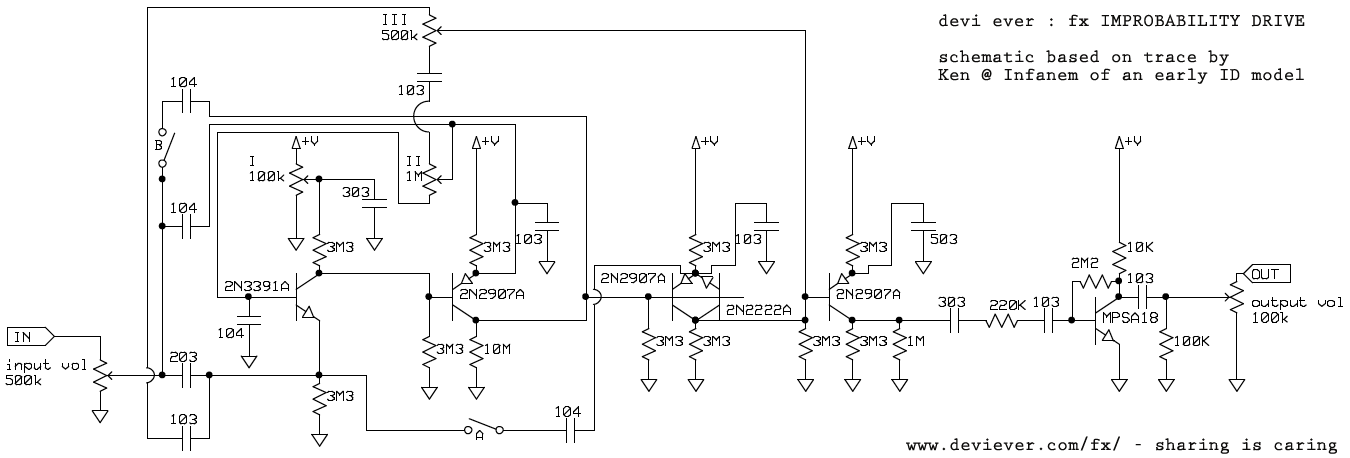
\includegraphics[width=1\textwidth]{improbdr}
	    \caption{The Improbability Drive, traced from a second version board, courtesy of Ken Schurer}
	\end{figure}
	
	\begin{figure}[H]
	  \centering
	    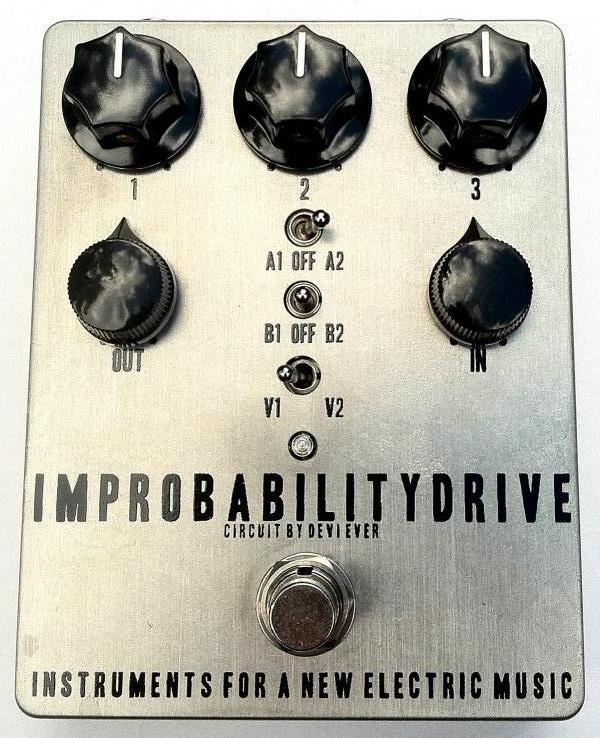
\includegraphics[width=.3\textwidth]{ID1}
	    \caption{The Improbability Drive, adapted for commercial production \citep{infanem}}
	\end{figure}
	
Following up on this project, user storyboardist designed a protoboard and circuit board layout and shares it with the rest of the thread. Astrobass and digi2t discuss the finer details of the modifications Schurer might have made to Devi Ever's original design. 

	\begin{figure}[H]
	  \centering
	    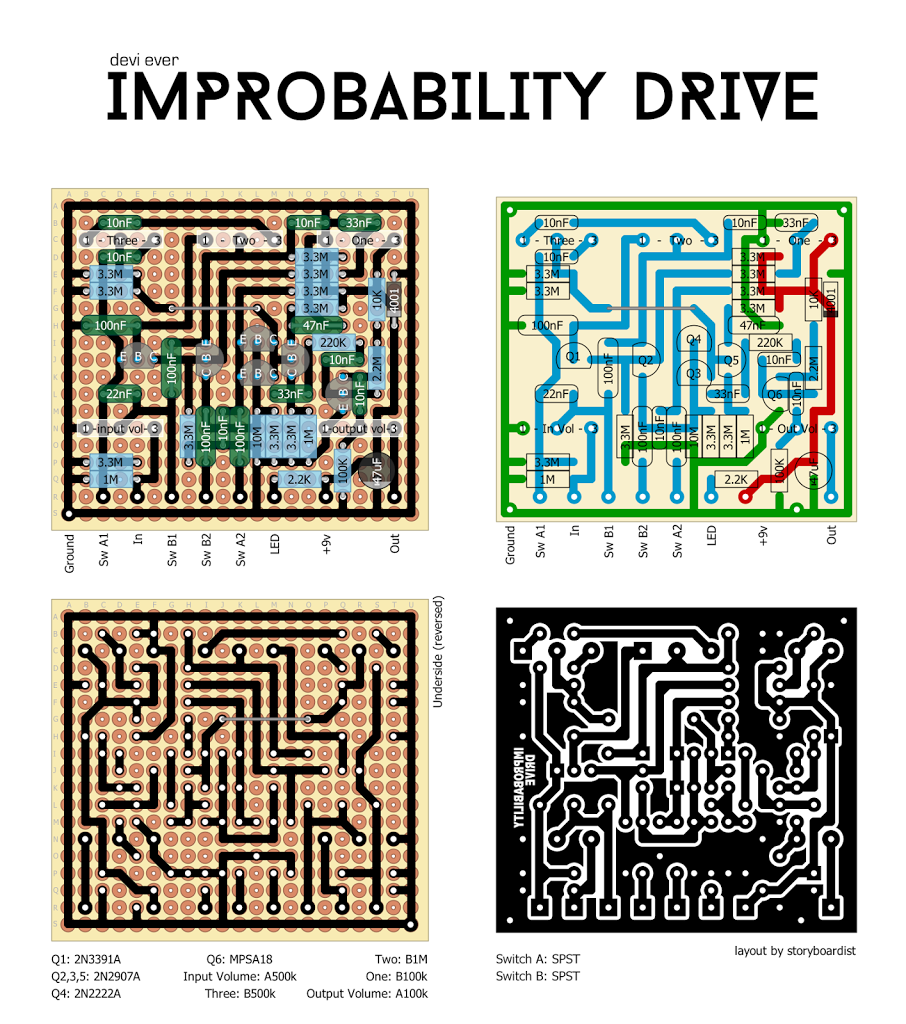
\includegraphics[width=.5\textwidth]{improbdr2}
	    \caption{The Improbability Drive circuit layouts for PCB or prototype board, courtesy of storyboardist}
	\end{figure}

In a couple of pages' worth of discussion, a discrete transistor fuzz circuit was resurrected and made easily implementable by anyone with 15 dollars worth of parts and a few hours of time, for no reason other than users appreciated Ever's original contribution and were willing to entertain another user's delayed interest \citep{freestomp}.

\begin{figure}[H]
	  \centering
	    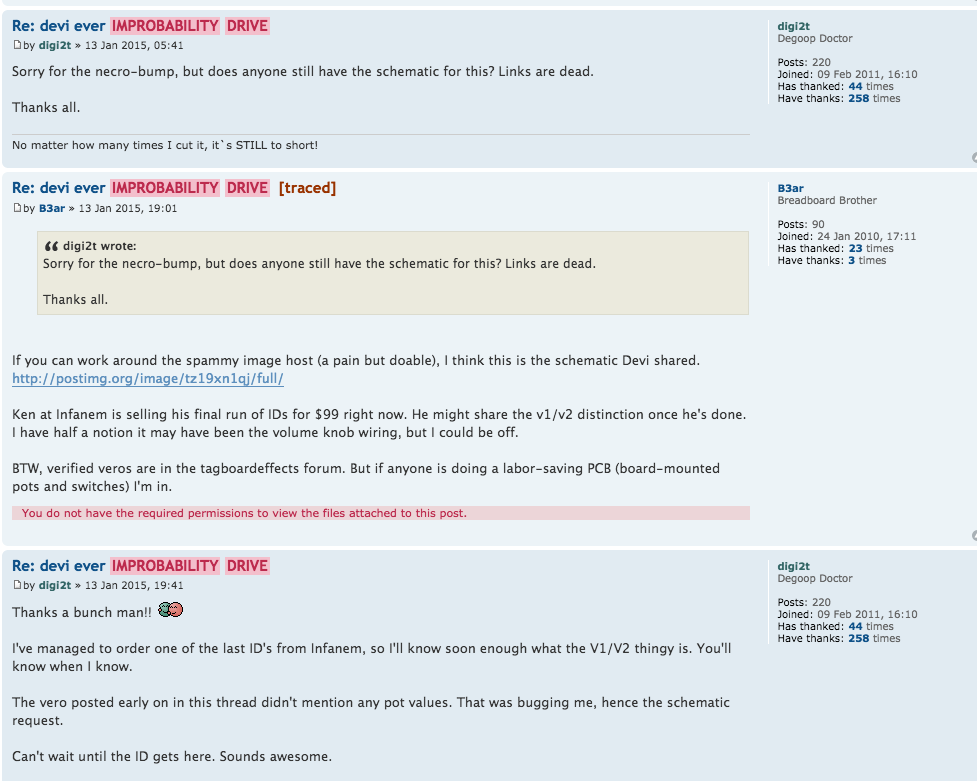
\includegraphics[width=1\textwidth]{freestomp}
	    \caption{a screenshot of the Freestompboxes.org page describing the \textit{Improbability Drive} \citep{freestomp}}
	\end{figure}

Presenting enough information to discuss a circuit design and replicate hardware results (in this case, timbres) is a typical maker practice, and constitutes the main source of content for websites like Hackaday, Instructables and portions of the Make Magazine website (as we'll see in a few sections). 

Other threads vary in detail. Some offer in-depth, component level analysis of each circuit, while other describe products so rare that there is barely any information on the topic. Unlike torrenting forums where rare catches are motivated by the concept of ratio bounty, users have little incentives to help other than curiosity and personal satisfaction. This website's audience is a dedicated, eclectic and usually friendly set of musicians and tinkerers united by an interest and a tool for sharing information. 

This example shows two things: first, that open approaches in electronic music hardware are still present today, and, second, that those open practices are in effect accessible to anyone with the resources and time to learn how to read a schematic in proximity of a soldering iron. Introductory projects such as this have two other consequences: encouraging the development of more sophisticated, personal projects, and serving as an educational gateway to circuits and notions of electrical engineering, design and  fabrication. 

\section{Jessica Rylan, \textit{Flower Electronics}}

Rylan's circuit design practices is based on both self-taught circuit skills and later rigorous training, either as an employee of Don Buchla's or later as a co-author with chaotic systems researcher J.C. Sprott \citep{piper2010}. In previous interviews, she expresses the unattractive formatted nature of classical approaches to additive or subtractive modular synthesis, as well as the generally male-centric communities behind it. This dissatisfaction is presented as a motivation for a number of circuit designs and corresponding commercial products \citep[pp.139-155]{rodgers2010}. 

Inspecting devices sold by her company, \textit{Flower Electronics}, over their period of operation (2006-2011) only imprecisely informs one of how this might have been done. Enclosures are still standard guitar pedal cases, albeit with layouts, knobs and banana patch jacks reminiscent of Buchla's designs. The underlying circuits roughly seem to follow modular synthesis architectures. A clear interest in chaotic oscillators is denoted, but even in that case, it seems difficult to break out of the VCO/VCF/VCA modular mold. 

In some sense, Rylan's work is at its most compelling when it is presented in the context of her own history and musical practice. The personal synthesizer, started in 2004, is the aptly named tool she developed in this quest of alternative design. 

\subsection{The \textit{Personal Synth} (2005)}

	\begin{figure}[H]
	  \centering
	    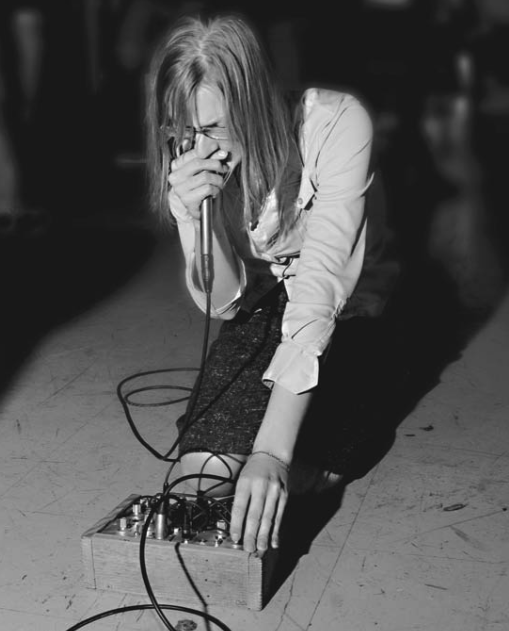
\includegraphics[width=.5\textwidth]{perssynth}
	    \caption{Jessica Rylan performing with the personal synth}
	\end{figure}
	
	\begin{figure}[H]
	  \centering
	    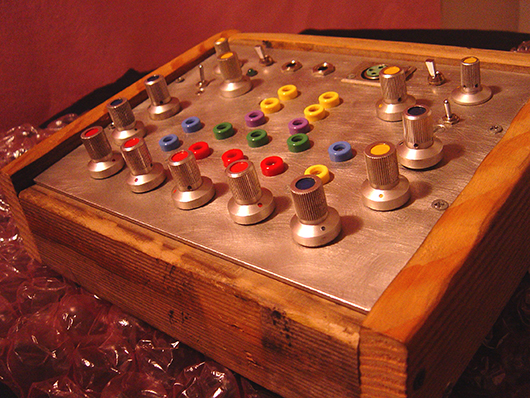
\includegraphics[width=.5\textwidth]{perssynth2}
	    \caption{The Personal Synth by Jessica Rylan, close up view courtesy of \citep{rylan2011}}
	\end{figure}
	
A particularly well documented instance of Rylan's work \citep{rylan2011}, this device is arguably the work that started Flower Electronics. Later commercial works by Rylan were not presented in such detail. 
	
Rather than paraphrasing the circuit analysis provided by Rylan, this section will comment on the devices originalities and their implications in the context of a hardware practice. 
	
At the heart of the device are two 8038 oscillator chips, in a doubled circuit Rylan derived from Thomas Henry's \emph{Audio Generator} \citep{rylan2011, henry} 

\begin{figure}[H]
	  \centering
	    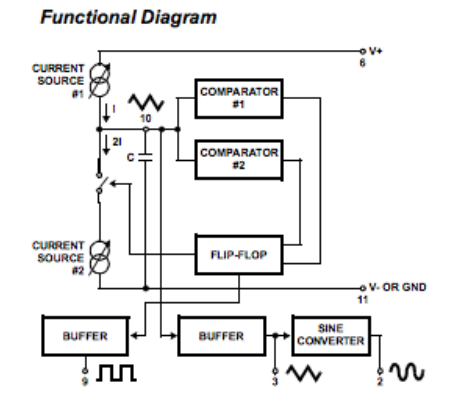
\includegraphics[width=.5\textwidth]{8038func}
	    \caption{The 8038 oscillator functional diagram, courtesy of Intersil}
	\end{figure}

Implementing voltage control of the wave-shaping section forms the basis for a versatile and compact device is unique: most timbral forming in analog synthesis takes place in the filter or modulation sections. 

\begin{figure}[H]
	  \centering
	    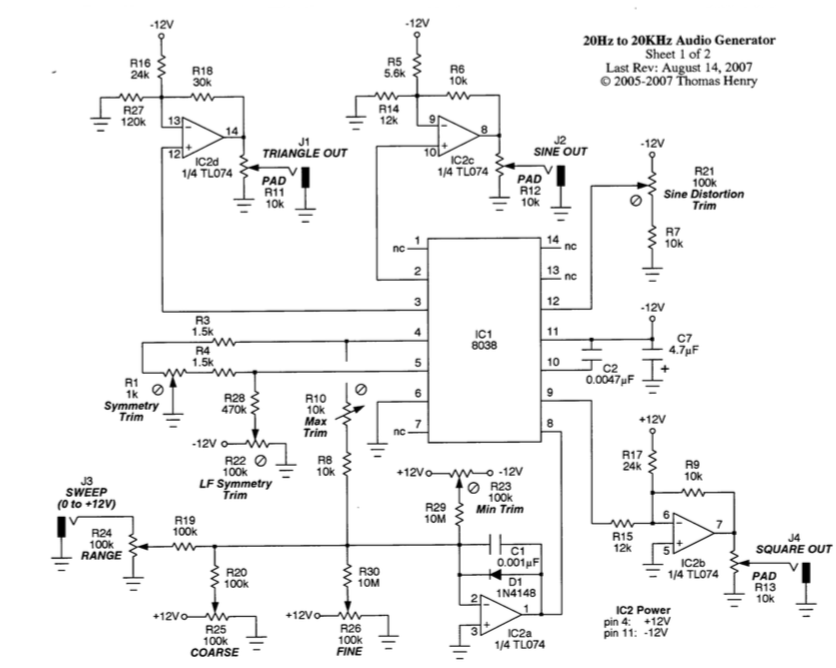
\includegraphics[width=1\textwidth]{s1}
	    \caption{The original 8038 oscillator schematic by Thomas Henry\citep{Henry}}
	\end{figure}
	
\begin{figure}[H]
	  \centering
	    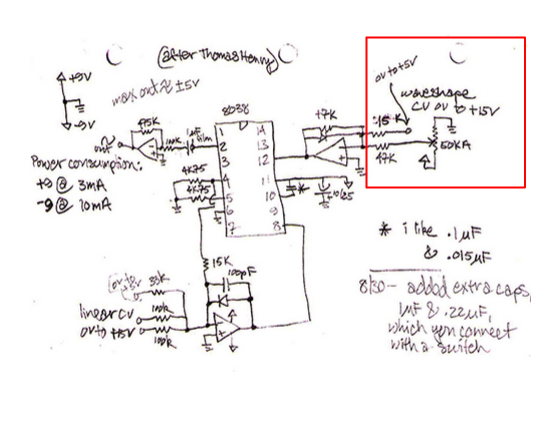
\includegraphics[width=1\textwidth]{rylanosc}
	    \caption{The \textit{Personal Synth}'s 8038-based oscillator\citep{rylan2011}. In red is the voltage controlled wave-shaper}
	\end{figure}
	
The choice of an 8038 is significant. By no means an antiquated design, the chip has however been discontinued as of writing, with no replacement from the manufacturer. As digital devices implement high quality sampling and the communications / military roots of semiconductor research lose interest in the specificities of chip oscillators, those designs get obsoleted at an increasing rate. Just like Nicolas Collins' 566 circuits, Rylan's 8038 circuit is a worthwhile study, but not necessarily the most practical avenue for the musical tinkerer.

This device is further expanded by a microphone input, in which the preamp produces low frequency oscillations if not turned off. Then, an original VCA implementing an unpredictable flavor of filtering through nonlinear zener diodes: 

\begin{figure}[H]
	  \centering
	    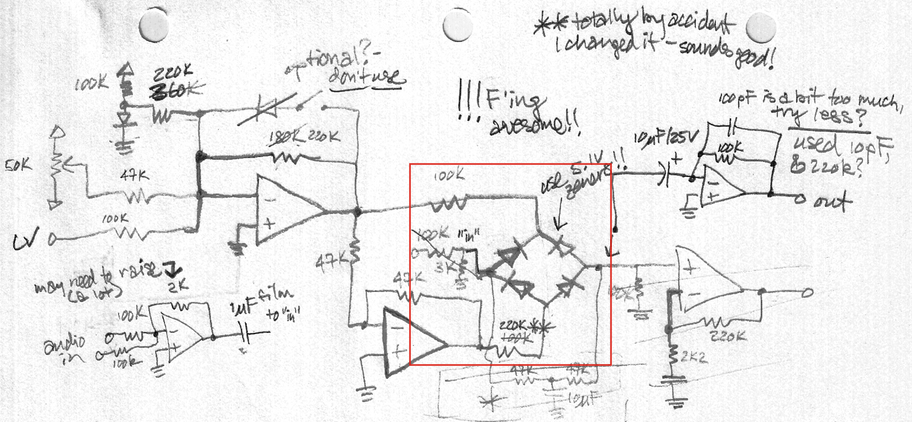
\includegraphics[width=1\textwidth]{rylanvca}
	    \caption{The \textit{Personal Synth}'s unique zener bridge VCA design. In red is the diode bridge for the VCA \citep{rylan2011}}
	\end{figure}
	
Rylan explains her reasoning behind this unusual choice of amplifier topology: 

\begin{quote}
	for the other really magic part of the personal synth, I eschewed filters and opted instead for a diode-bridge VCA, implemented with zener diodes. Theoretically the Zener shouldn't really change things (consider how attenuated the audio input it) but as they say, the results speak for themselves.
\end{quote}

\citep{rylan2011}

For a high-level view of the device, she offers the following diagram: 

\begin{figure}[H]
	  \centering
	    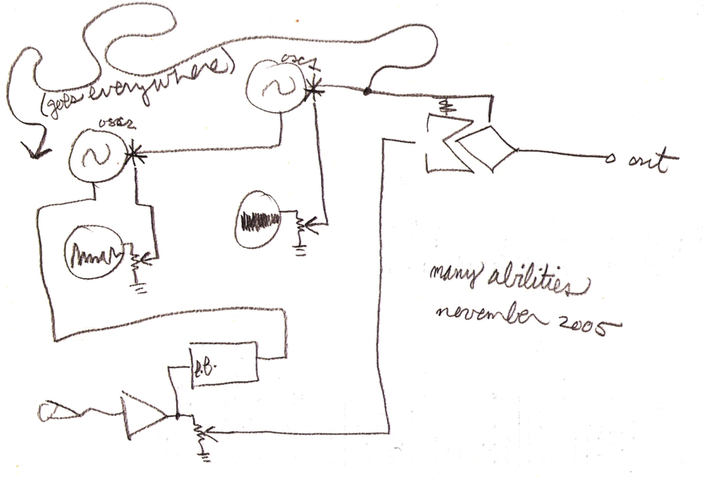
\includegraphics[width=1\textwidth]{rylanfunc}
	    \caption{The functional diagram for the \textit{Personal Synth} \citep{rylan2011}}
	\end{figure}
	
After some reworking, a typical patch might involve the following clarified signal flow: 

\begin{figure}[H]
	  \centering
	    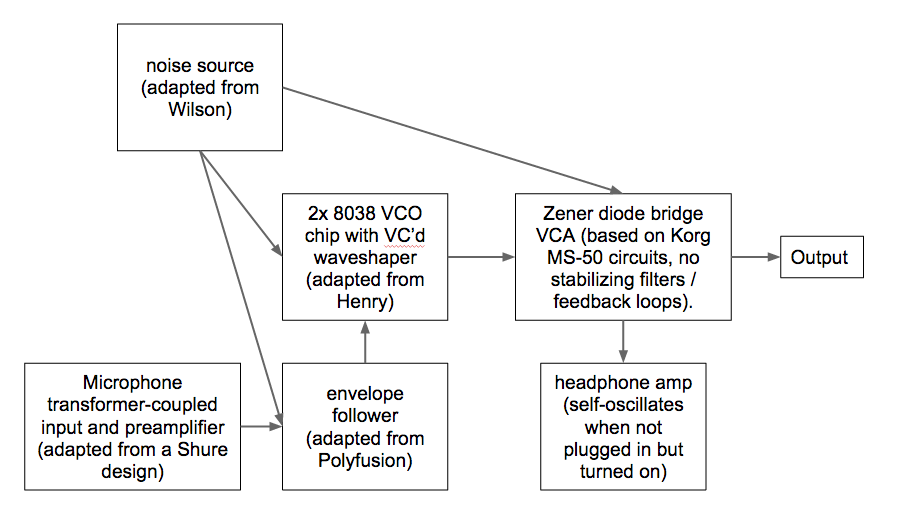
\includegraphics[width=1\textwidth]{ezrafunc}
	    \caption{The adapted functional diagram for the \textit{Personal Synth}}
	\end{figure} 
	
If the Personal Synth is perhaps not a completely new way to think about analog synthesis, it was a new way for Rylan to think about music which prompted the development of successful business. A number of the decisions within the device, such as removing feedback capacitors and protections or including differently nonlinear devices at crucial elements, all constitute instances of post-optimal design, meant to enhance the poetic capacities of the device. This post-optimality and chaotic behavior links Rylan to Tudor's concept of letting electronics speak for themselves.  

\section{Ben Hinz: \textit{Dwarfcraft Devices}} 

\begin{quote}
	
	We can make our ``1"-``0" decisions into just about anything- a musical note, a test waveform, a measured and displayed value, a video presentation, a clock, a game, an industrial control, a toy, a microcomputer, an art form, a community information access service, or just about anything else you can dream up. All it takes is the right number of logic blocks properly connected to do the job.
	\citep[pp-7-8]{lancaster1988}
	
\end{quote}

\emph{Handmade Electronic Music} focuses much of its circuits around the Complementary-Silicon-Metal-Oxide (CMOS) family of integrated circuits. Collins acknowledges inspiration from Lancaster's \textit{CMOS Cookbook}, quoted above. In doing so, both authors recognize how powerful binary information - an its continuous counterpart, the square wave - can be in relatively simple synthesis environments. Older examples abound: the Weird Sound Generator, a typical first synthesis project sold as a kit by Ray Wilson from the \emph{Music From Outer Space} website, relies on interconnected CMOS chips for its synthesis \citep{wilson2015}. \textit{Beavis Audio}, an important DIY music website, focuses one of its most interesting blog posts on this family of circuits, naming Collins as an influence \citep{beavis2015}. 

Although Collins is not the only source of these digital logic sound generators, the publication of his book has had a visible impact on many of the low-part-count synthesis circuits seen today. The following examples exhibit particularly interesting and relevant projects, as Ben Hinz acknowledges that he started making audio electronics based on the Collins book (personal exchange, 2015)

\subsection{The \textit{Robot Devil} (2012)}

The Robot Devil is an octave and distortion instrument effect based around two integrated circuits from the 4000 family of CMOS chips, the 4040 clock divider and the 4049 hex inverting buffer. Just like with the \textit{Improbability Drive}, a forum post contains most of the information necessary to analyze the device to the component level \citep{freestomp2}. 

Similar 4049 circuits are presented in Craig Anderton's classic \emph{Electronic Project for Musicians} \citep[p.173]{anderton1980}, then updated by in Collins' \emph{Handmade Electronic Music} \citep[p.155]{collins2006}, with Poss' law as subtitle: \emph{Distortion is Truth}.

As one can see from the forum schematics provided by user \emph{nocentelli}, the \textit{Robot Devil} distortion portion of the circuit appears to be closest to the original Craig Anderton version, rather than Collins' augmented 3 buffer or distortion+fuzz versions:

\begin{figure}[H]
	  \centering
	    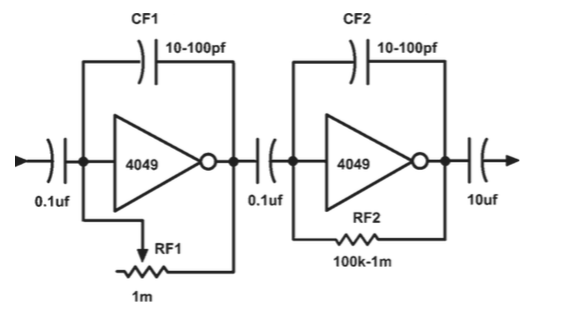
\includegraphics[width=1\textwidth]{nicdist}
	    \caption{Two stage distortion schematic by Collins \citep[p.155]{collins2006}}
	\end{figure} 

\begin{figure}[H]
	  \centering
	    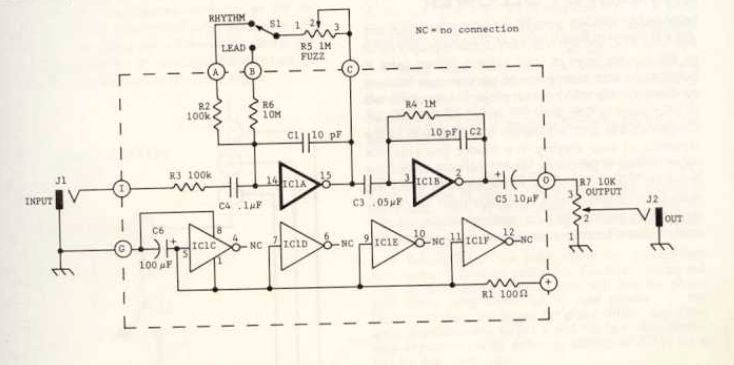
\includegraphics[width=1\textwidth]{tubedist}
	    \caption{A ``tube sound fuzz schematic'' by Anderton \citep[p173]{anderton1980}}
	\end{figure}

\begin{figure}[H]
	  \centering
	    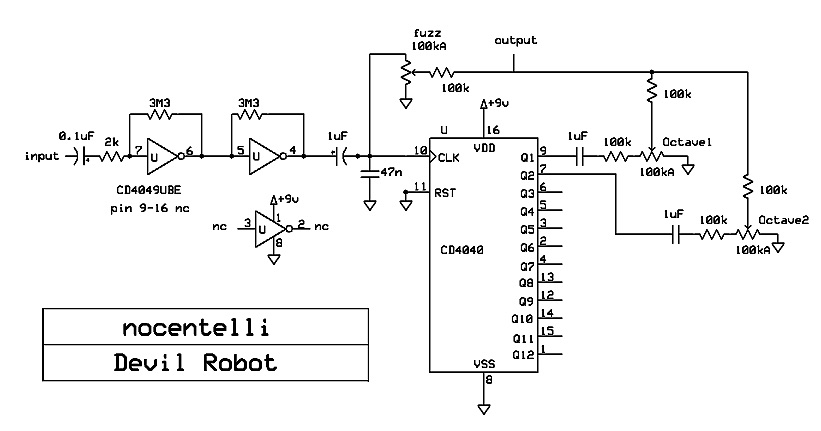
\includegraphics[width=1\textwidth]{robotdev}
	    \caption{The \textit{Robot Devil} schematic, as traced by user Nocentelli \citep{freestomp2}}
	\end{figure}

The 4049 circuit is based around using this hex inverter/buffer integrated circuit as a linear amplifier. Since the buffering components are designed around field effect transistors (FETs), overdriving one of the six buffers it contains with another used as an amplifier causes tube-like distortion without having to deal as explicitly with discrete FET circuit design \citep{nishizawa1974}. 

The gain around each amplifier stage is set by the ratio between the loop resistor, Rf and the input resistor, Ri. In this case, the gain is extremely high (more than 20 000, which means that even a small input signal with distort the output of amplification stages to the extremes of what the power supply can provide before the signal reaches the 4040 divider chip. 

The 4040 then acts as an ``analog'' octave effect. As user \emph{Jonasx24} mentions, the 4020, 4024 and 4040 are all designed to perform similar division roles, taking in square waves of a certain frequency and outputting multiples of that frequency. This is particularly useful in digital circuits, but also in audio: if a distortion circuit can provide an incoming audio signal with enough higher harmonics to appear as a ``square wave'' to the divider circuit, it'll produce octave of the incoming signal. In our case, the outputs chosen correspond to the octave down from the input (divide by two) and two octaves down from the input (divide by 4). Looking at the 4040 divider circuit in \emph{Handmade} \citep[p.159]{collins2006}, we can see how close \emph{nocentelli}'s circuit is to Collins' \emph{Low Rider}: 

\begin{figure}[H]
	  \centering
	    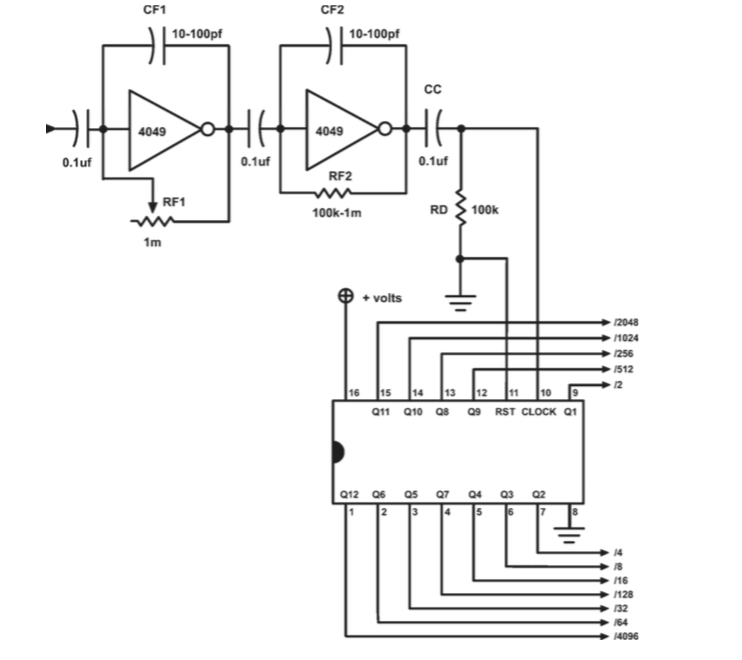
\includegraphics[width=1\textwidth]{lowrider}
	    \caption{The \textit{Low Rider} schematic by Collins \citep[p.159]{collins2006}}
	\end{figure}

Here, CMOS chips are misused into serving as functional instrument signal processing devices. Similar commercial octave effects such as \textit{Electro-Harmonix}'s \textit{Octave Multiplexer} show that even with low gain, dividers can be used to semi-accurately track and shift octaves for incoming signals. 

\begin{figure}[H]
	  \centering
	    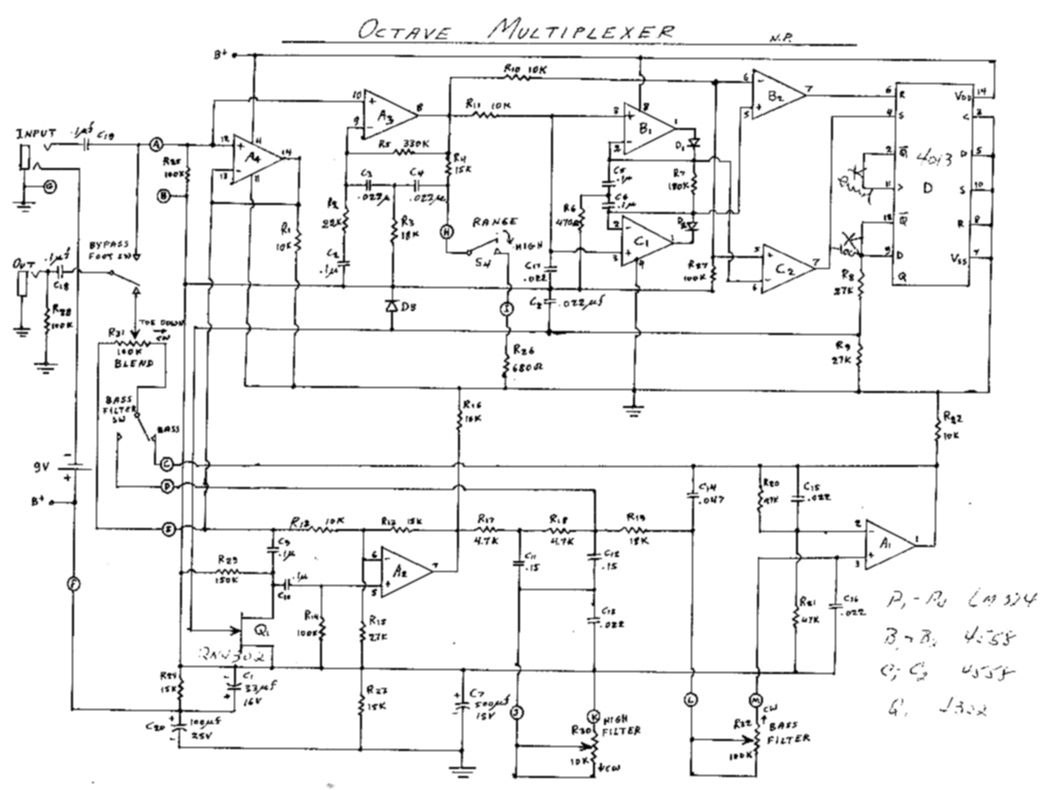
\includegraphics[width=1\textwidth]{octmux}
	    \caption{The \textit{Octave Multiplexer} schematic by \textit{Electro-Harmonix} \citep{}}
	\end{figure}
	
To resume this device into its main components, a simple annotated version of nocentelli's original schematic suffices: 

\begin{figure}[H]
	  \centering
	    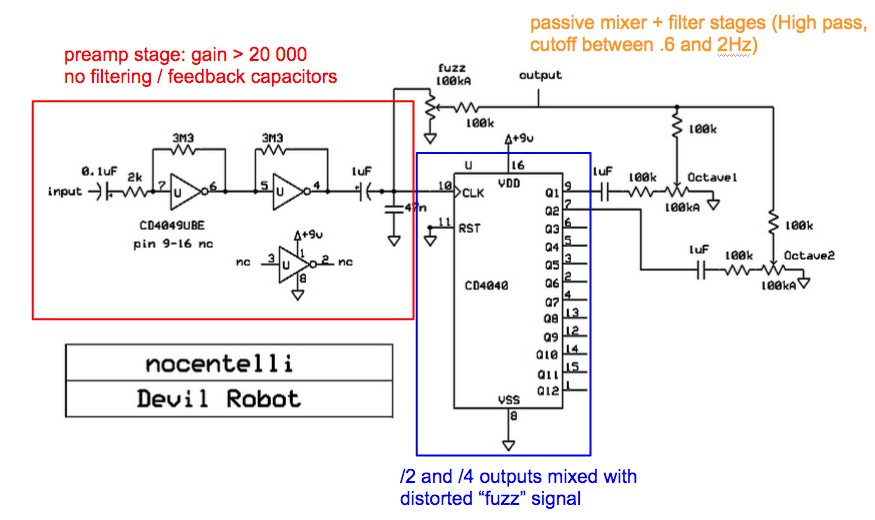
\includegraphics[width=1\textwidth]{robdevexpl}
	    \caption{The annotated version of the\textit{Robot Devil} schematic by \textit{Nocentelli}}
	\end{figure} 

Just as in the case of the \emph{improbability drive}, forum users were provided with enough information by the original poster to make the details of the Dwarfcraft design of little practical importance, even if it could have potentially been more refined. As Martin Howse mentions in his interview, proprietary designs often forces creative minds to solve the same problem multiple times. In this case, more than solving a problem, users have assembled a replacement circuit from pre-existing work and experimentation - in short, they've hacked a circuit and made it their own. 

In this case, the 4040 chip reacts erratically when the signal decays and upper harmonics come to be of equal amplitude as that of the fundamental for single notes, or when chord components decay less quickly than the chord's root note. In our case, Hinz did took out most of the linearizing and stabilizing components recommended by Anderton and Collins. This is often what makes such effects chaotic and to some, interesting. This is a clear example of a post-optimal device, squarely in the lineage of Collins' practice and teachings. 

\section{Taylan Cihan}

Taylan Cihan was a Cornell electroacoustic music center graduate student who undertook a variety of electronic music hardware projects \citep{taylan}. \textit{Porcupine} was developed using scraps from his previous project, \textit{Vermes}. Cihan was in the process of developing a student space dedicated to the fabrication of electronic hardware for music. Some of the information here was provided by his late advisor and close collaborator Professor Kevin Ernste. 

\subsection{\textit{Porcupine} (2013)}

\begin{quote}
	
	After being stabbed numerous times by the wires sticking out of the device while building it, the name, Porcupine, came out rather naturally. Porcupine, as I would like call, is a concrète box (in reference to musique concrète), combining a built-in analog sound processor with a variety of acoustic sounds that can be generated using the wires. The copper plate and wires are essentially leftover parts from my previous project, Vermes. Instead of throwing it all away, I have decided to recycle them, hence the faint artwork on the surface of the plate, a by-product of my failed very first attempt at making my own PCB.

	The sound processor include an analog delay, fuzz distortion, and resonating low-pass filter. A piezo element attached to the copper plate picks up the sound of the wires, which is amplified through a high-gain preamp before sent to the processing unit. An additional 1/4" jack input, which also has its own high-gain preamp, allows the device to be simultenously used as an effects unit to process the external sounds. When the levels, delay time, fuzz gain and filter resonance set to a maximum, the circuit starts to self-oscillate, producing a rich harmonic spectrum.
	
	\end{quote}
	
	\citep{cihan2015}
	

Taylan Cihan's \textit{Porcupine} is included here because it serves as an elegant example of what experimenters who've grown comfortable with the various components of standard circuits such as those presented in \emph{Handmade Electronic Music} can do. Higher-level combinations of circuits along with unique interfaces are often the logical next step to making more compelling instruments. In this case, Cihan achieved success by combining semi-standard circuits with an inside-out interface in order to embrace the chaotic experiments from which inspiration came. 

Specifically, Cihan's circuit is based on the following building blocks: 
	
\begin{quote}
		
The delay unit is built using a PT2399 Echo Processor IC by Princeton Technologies.

Fuzz distortion is a clone of EHX Muff Fuzz. Schematic from Beavis Audio.

The 4049 Hex Inverter preamp schematic is from Nick Collins' Handmade Electronic Music book (p.187).
	
	\end{quote}

	\citep{cihan2015}

	\begin{figure}[H]
	  \caption{The \emph{Porcupine} by Taylan Cihan, front view}
	  \centering
	    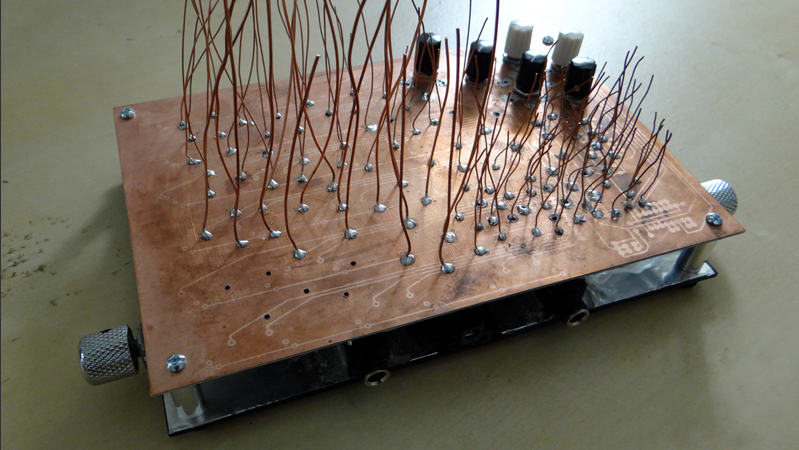
\includegraphics[width=.5\textwidth]{porcupinetop}
	\end{figure}
	
	\begin{figure}[H]
	  \caption{The \emph{Porcupine} by Taylan Cihan, circuit board view}
	  \centering
	    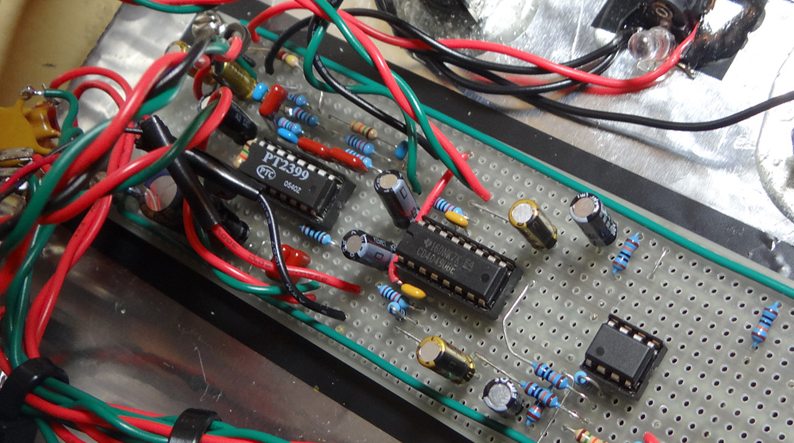
\includegraphics[width=.5\textwidth]{porcupinein}
	\end{figure}
	
The circuit board view shows three integrated circuits: a PT2399, a 4049, and a eight pin DIP package IC.

The 4049 is a CMOS Hex Inverter used as a resonating low pass filter, based on one of Nicolas Collins' designs.

	\begin{figure}[H]
	  \caption{Nicolas Collins' 4049 Low Pass Resonating filter from \emph{Handmade Electronic Music}}
	  \centering
	    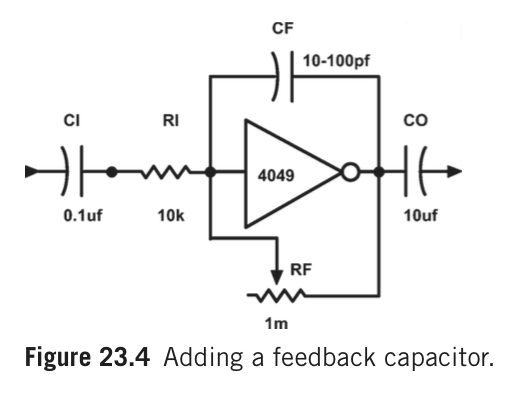
\includegraphics[width=.5\textwidth]{4049lpf}
	\end{figure} 
	
As detailed in the previous chapter, this circuit and its associated notes are available in the public draft for \emph{Hardware Hacking}. 

	\begin{figure}[H]
	  \caption{Nicolas Collins' 4049 Low Pass Resonating filter from \emph{Hardware Hacking}}
	  \centering
	    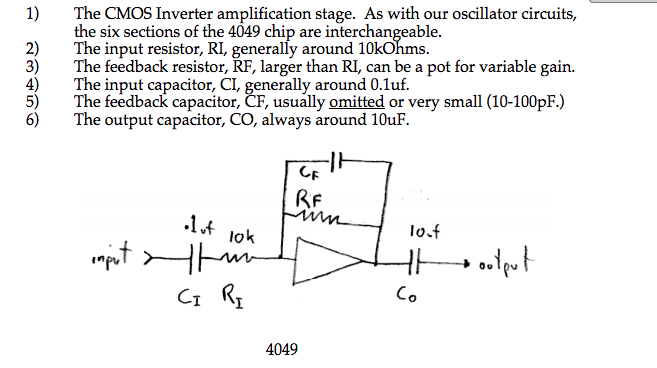
\includegraphics[width=.5\textwidth]{4049lpf2}
	\end{figure} 

The PT2399, with two electrolytic capactitors, seven mylar capacitors and eight resistors, appears to be a variation on the stock circuit from the PT2399 application note.

	\begin{figure}[H]
	  \caption{PT2399 stock circuit, from the application note by Princeton Technologies}
	  \centering
	    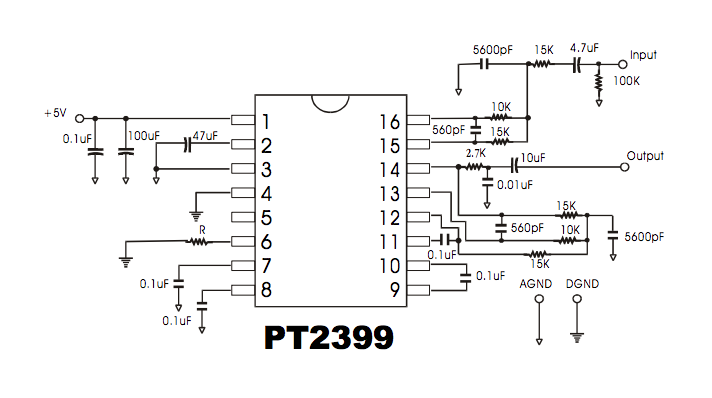
\includegraphics[width=.5\textwidth]{pt2399circ}
	\end{figure}
	
The Muff fuzz circuit is based on an original Electro-Harmonix design as traced by Beavis Audio \citep{beavis2015b} . It is a classic of distortion circuits, a simple and expressive two transistor design which gave Electro Harmonix its reputation. Its parts are common and inexpensive, with various DIY vendors offering kit versions with extremely detailed assembly instructions.

	\begin{figure}[H]
	  \caption{Beavis Audio Muff Fuzz}
	  \centering
	    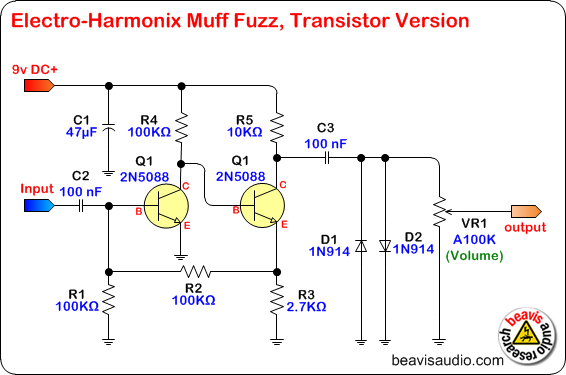
\includegraphics[width=.5\textwidth]{mufffuzzbeavis}
	\end{figure}
	
The third chip, although illegible in the picture above, is probably an op-amp IC used for the piezo preamp Cihan mentions. 

In effect, this combination of circuits and hardware is a versatile, expressive and personal approach to exploring the possibilities of audio circuits. It is simple enough to be understood in two paragraphs, two links and one reference, but the result is arguably greater than the sum of its parts. This is especially due to the nature of the interface, the ability of the device to both process and generate, and the re-use of materials from a previous project. By exposing the mess of wires and their prickly unfriendliness, Cihan exhibits his appreciation for his medium of choice. This interface design can be considered post-optimal: mild pricks caused from playing with the exposed, sharp wire definitely fit within Dunne's vision of ``user-unfriendliness''. This unusual, personal approach to developing an electronic instrument would seem inconvenient to anyone looking for a synthesizer, but to anyone else who's tinkered with electronics, the description of the project's genesis and the corresponding result will make perfect sense. 

This is where hardware design can ask greater questions in the field of music performance and sound art. The sculptural aspect of the device is indirectly reminiscent of sonic installations by Tudor, Lucier and their aesthetic descendants.\emph{Porcupine}'s ability to both generate and process sounds greatly enhances its potential to be part of a larger, evolving system. By sharing this design, Cihan quietly kept experimental ideals alive. By keeping the information incomplete, he also encouraged exploration and personalization: in effect, Cihan and his peers allow for open musical hardware to go from self-sustaining to self-expanding. 

Cihan details the PT2399 delay chip as an analog one. Indeed, the Princeton Technology Corporation datasheet identifies it as an ``echo audio processor IC utilizing CMOS technology which is equipped with ADC and DAC, high sampling frequency and an internal memory of 44k.'' \citep{princetonpt} It is a good example of what followed basic logical operators of the 4000 series introduced with the \textit{Robot Devil}.

	\begin{figure}[H]
	  \caption{The PT2399 internal block diagram from the Princeton datasheet}
	  \centering
	    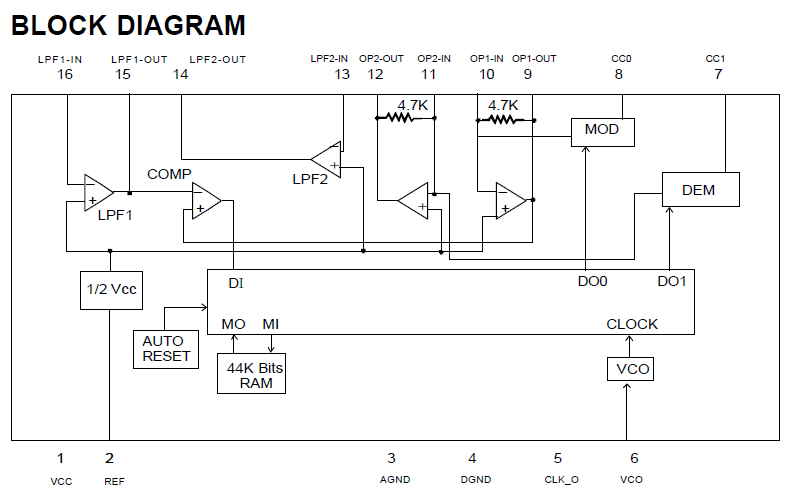
\includegraphics[width=.5\textwidth]{pt2399diag}
	\end{figure}

By combining large numbers of microscopic scale logical operators and connecting those to memories and clocks, CMOS sampling ICs such as this one are possible. The chip is occasionally labeled as analog (sounding convincingly so) by various manufacturers and DIY guides - this suggests that Cihan gathered information from other experimenters online, making him a public participant in the field of open musical hardware design. The next level of complexity in integrated circuits is, arguably, microcontrollers. 
 
\section{Tristan Shone}

The PT2399's main limitation is its relatively small set of applications: generating delayed copies of the input signal within certain limits of amplitude, delay and current draw. 

As other subcomponents of computing systems followed in the process of miniaturization, small and accessible systems have become ubiquitous in the arts because of their versatility: microcontrollers. Of particular interest in the arts and this discussion in particular is the Arduino hardware and development environment \citep{gibb2010}. The Arduino usually uses an IC from the AVR family: 

	\begin{figure}[H]
	  \caption{The AVR system block diagram for the ATMega328, from Atmel - included in the recent Arduino packages}
	  \centering
	    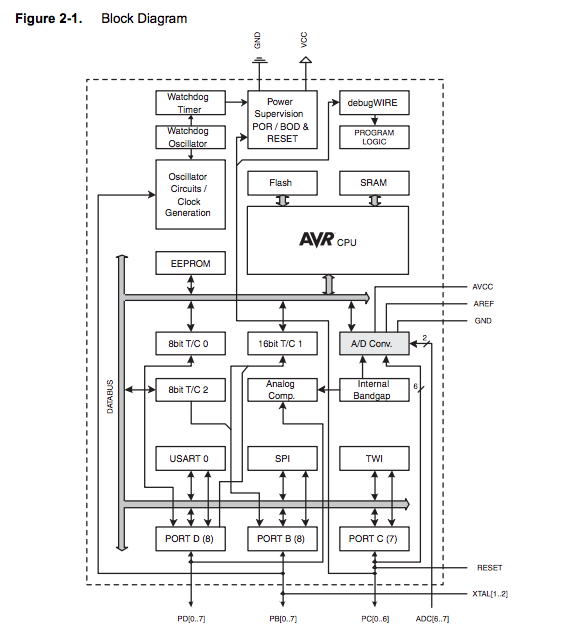
\includegraphics[width=1\textwidth]{avrarch}
	\end{figure}

In recent years, the large variety of Arduino packages have had a particularly strong impact on creative computing in sound and installation work. Presenting those here allows a discussion of various custom-made instruments which exhibit innovations at various levels and represent additional visions of post-optimality in electronic music instruments. 

Tristan Shone has a musical practice based around microcontrollers and goes under the name \emph{Author and Punisher}. 

A mechanical engineer and sculptor, Shone is the musician responsible for this one-man project. He released a first album in 2005, \emph{The Painted Army} \citep{shone,2005}, as he was developing his first set of instruments, the Drone machines. His website's subtitle is ``electromechanical destruction since 2004'' \citep{shone2004}.

	\begin{figure}[H]
	  \centering
	    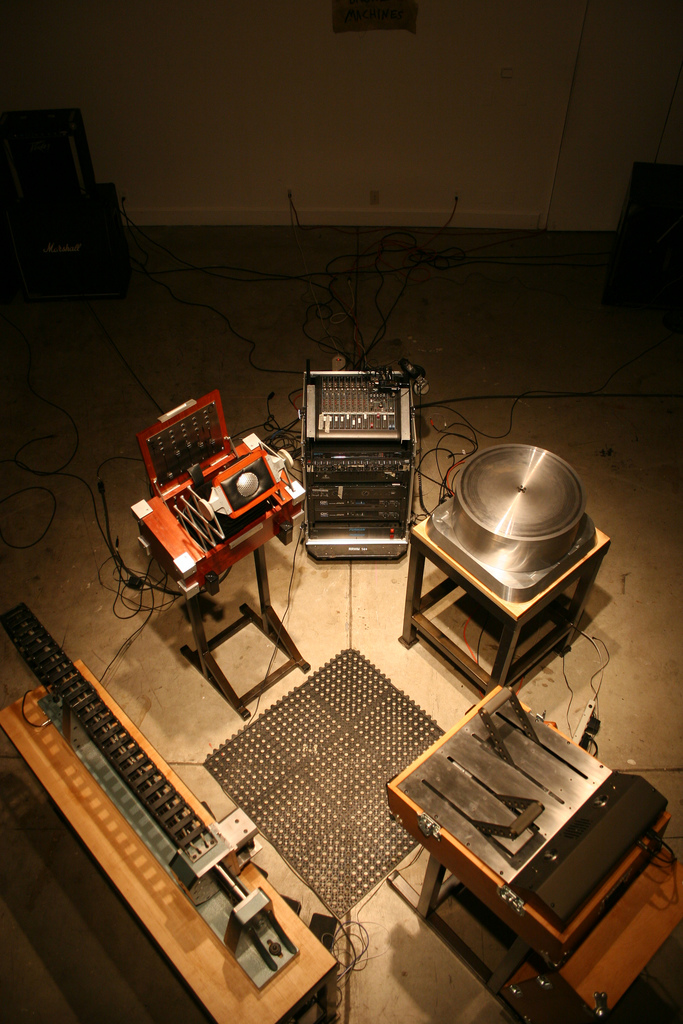
\includegraphics[width=.5\textwidth]{drone}
	     \caption{Tristan Shone's live setup around the release of the \emph{Drone Machines} album, courtesy of Shone}
	\end{figure}
	
He has since released three more full-lengths relying increasingly on hardware he fabricated, in conjunction with a software sampling and synthesis system built around Ableton Live. Most of his devices have evocative names such as \emph{Linear Actuator}, \emph{Big Knobs} or \emph{Bellows}. 

	\begin{figure}[H]
	 	  \centering
	    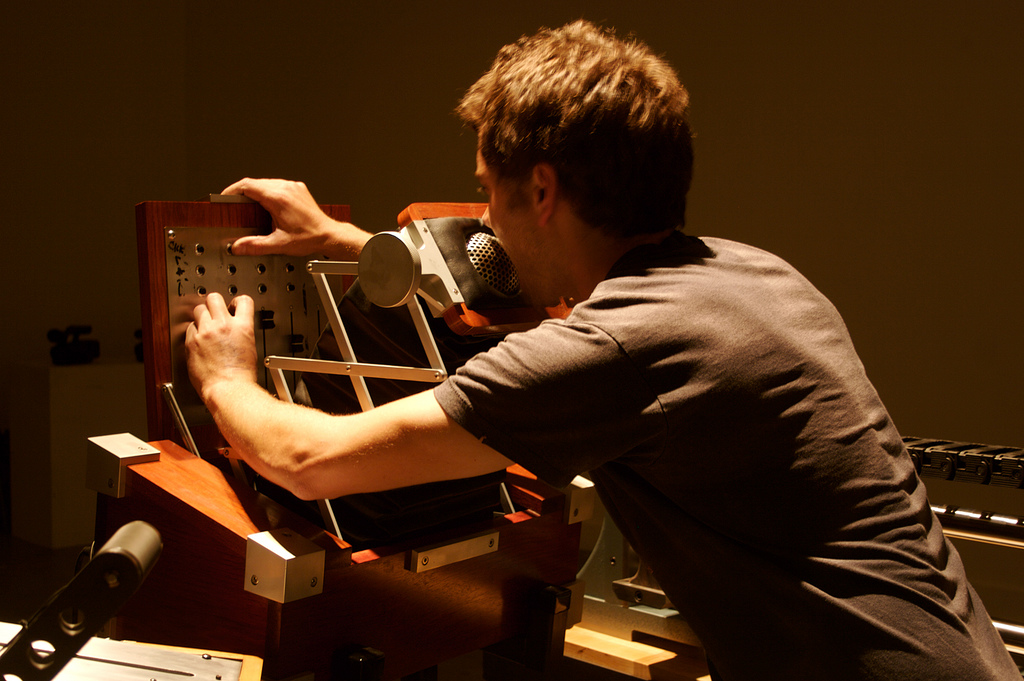
\includegraphics[width=1\textwidth]{bellows}
	    \caption{The \emph{Bellows} instrument, made by Tristan Shone, courtesy of Shone}
	\end{figure}

His experience with sculpture and mechanical engineering are clear, although discussing the matter with him makes it clear that he is ultimately making those because they seem like the best way to perform his music. Although he has grown to try and move away from the visual impact of his setup by collaborating with visual artists, his website still provides the curious with a combination of evocative live shots and technical diagrams. 

	\begin{figure}[H]
	  	  \centering
	    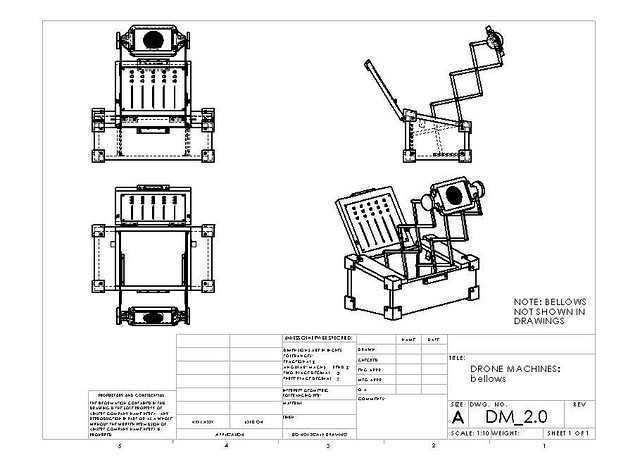
\includegraphics[width=1\textwidth]{bellowsdiag}
	    \caption{The technical diagram for the \emph{Bellows} instrument, courtesy of Shone}

	\end{figure}
	
Most of these electromechanical devices act as controllers: they encode movement into a number using Arduino systems. This information is then fed into a computer, which triggers starts, changes and ends for specific sets of pre-composed sounds. 

Shone's microcontrollers system is based on the Arduino environment, which he uses with custom firmware developed by Dimitri Diakopoulos and featured at NIME in 2011 \citep{diakopoulos2011,diakopoulos2015} . This firmware modification turns a specific strands of the Arduino hardware (the Uno, Due and Mega 2560 boards) into a driverless device, enabling it to send MIDI data over USB without any more setup than a commercial USB-MIDI item. 

However, Shone's live setup is not just centered on controllers. Shone describes himself as a ``lifelong beatboxer'' and in this context, he's devised a number of ways to detect, record and manipulate his voice \citep{shone2012}. He's currently developing a set of masks (documented on his website are the trachea quad mic, the dither mask, the drone mask and the mute mask), while his previous vocal interface is called the Headgear. That system was the topic of a tutorial written by Shone for the Make Magazine website \citep{shone2012}, and uses electret microphones. 

\subsection{ \textit{Headgear} (2011)}

	\begin{figure}[H]
	  \centering
	    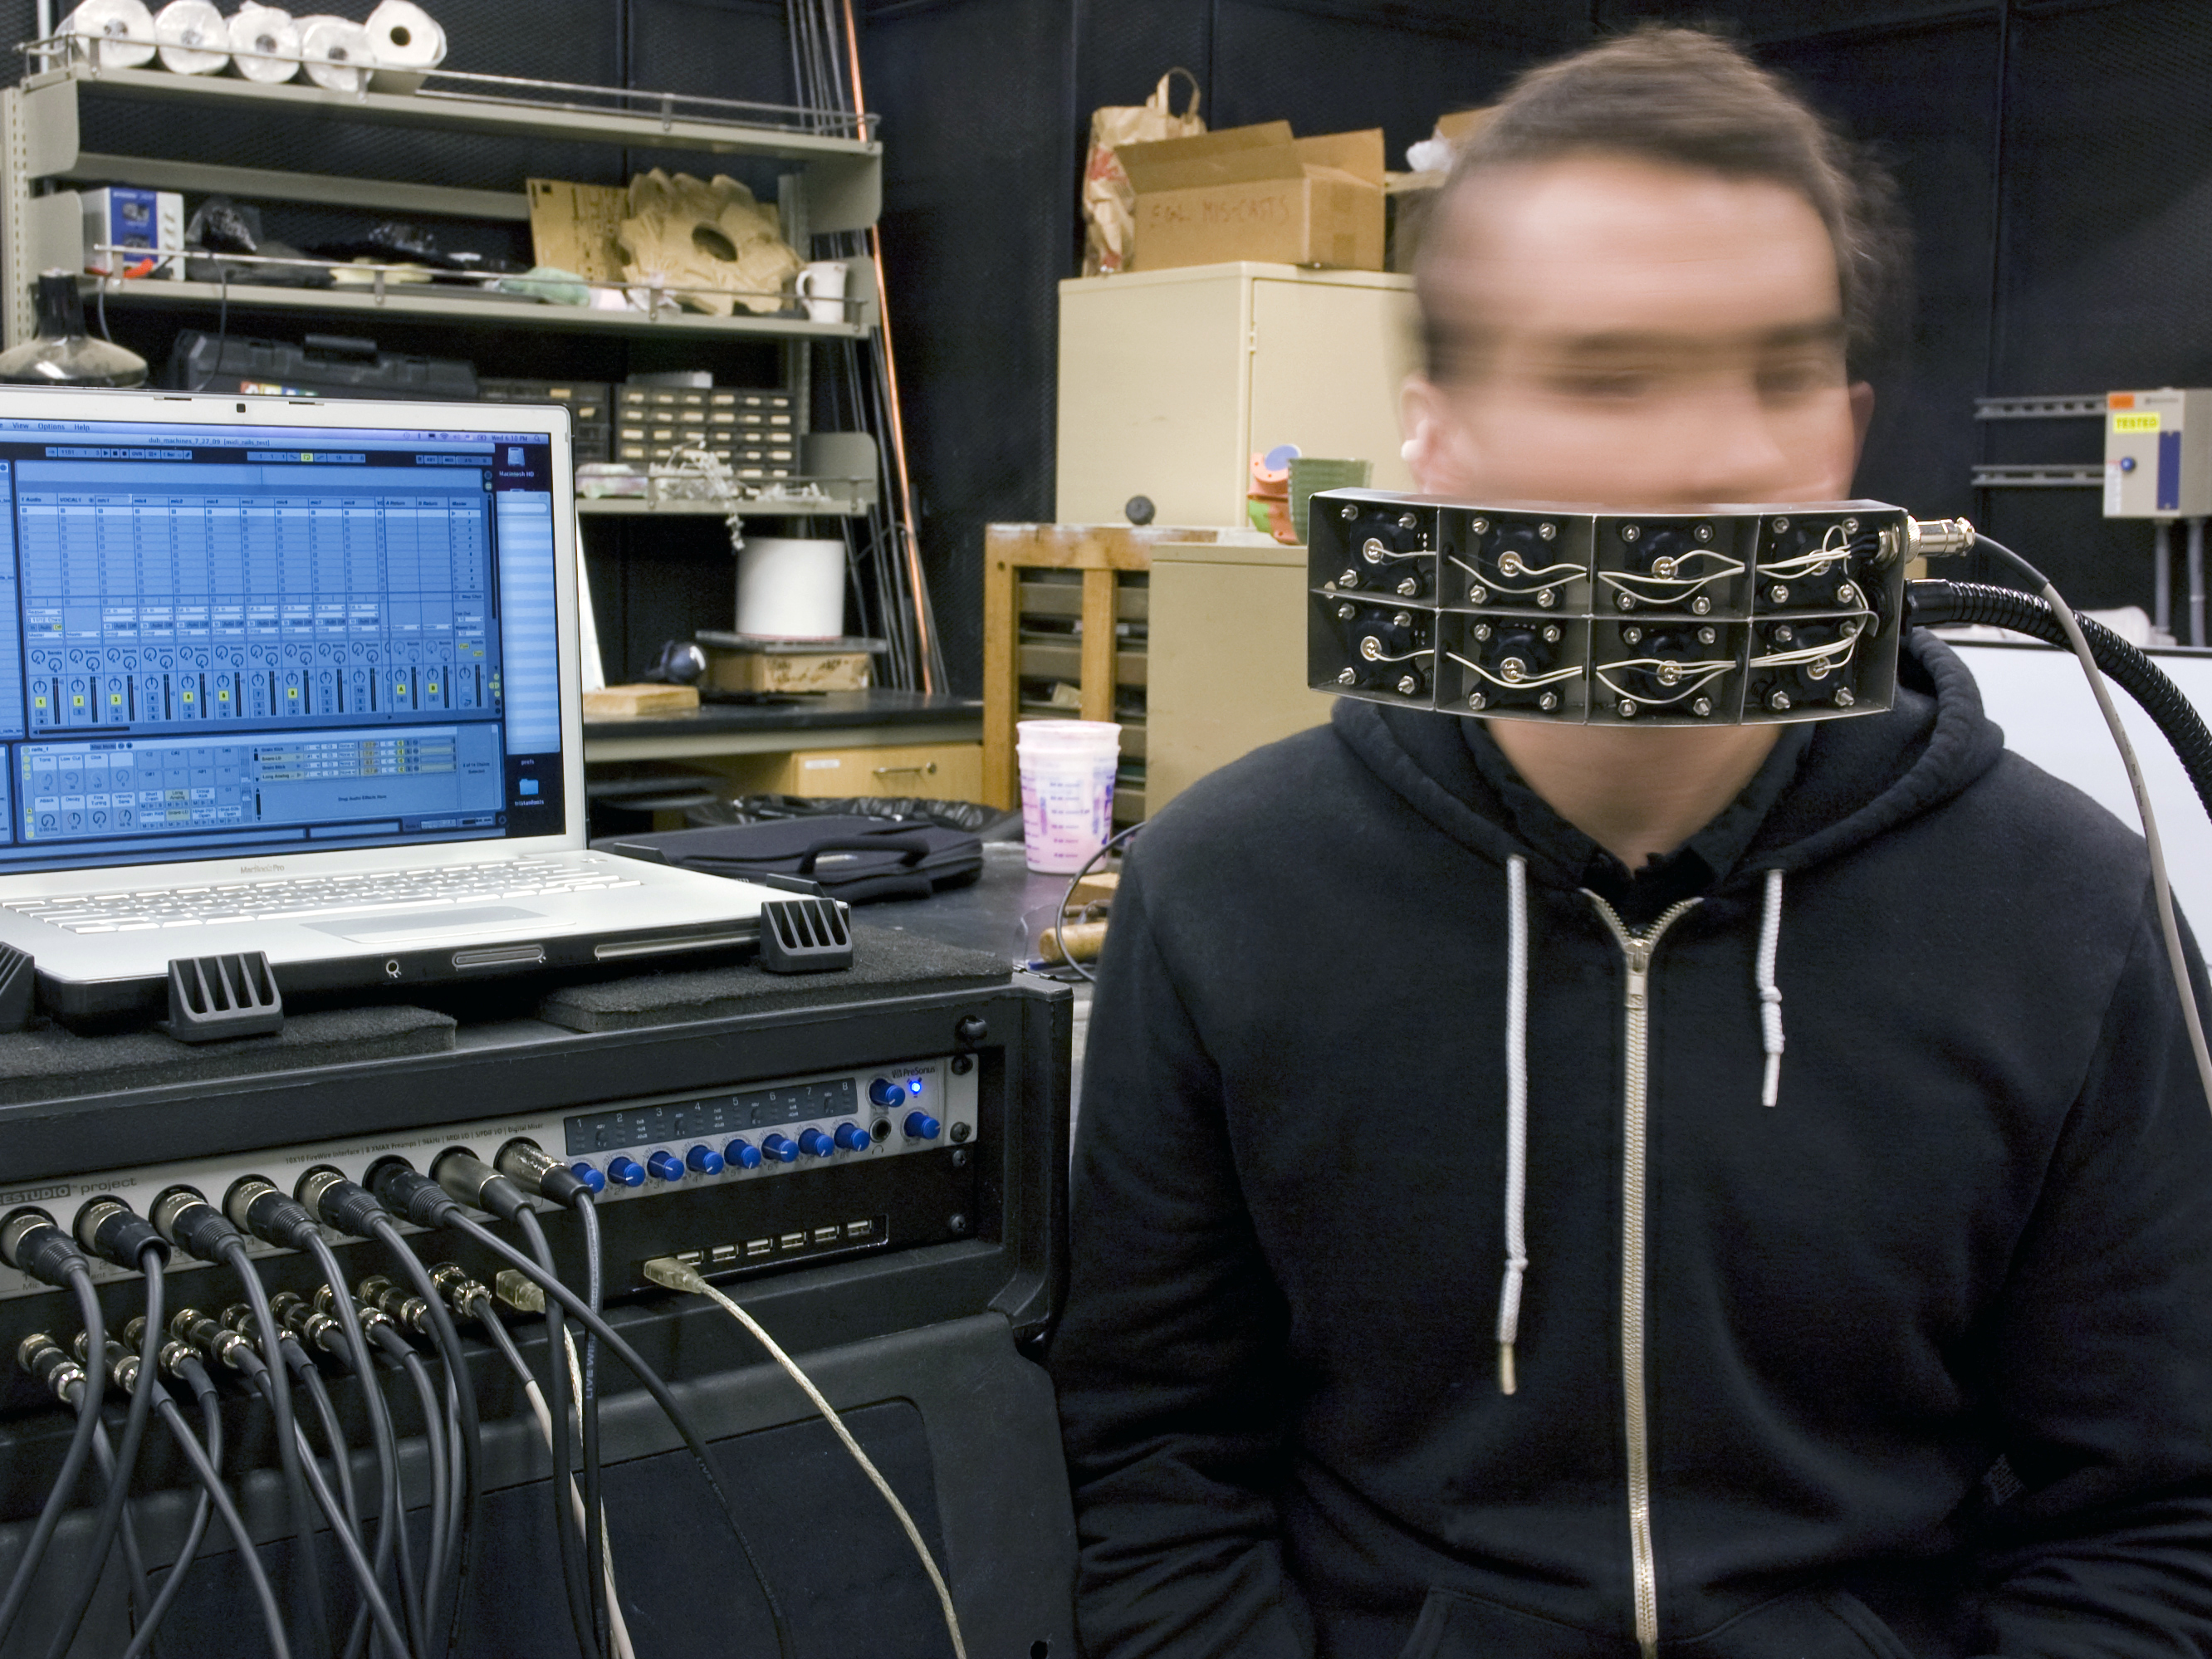
\includegraphics[width=1\textwidth]{headgear}
	     \caption{The Headgear device by Tristan Shone, wired for operation, courtesy of Shone}
	\end{figure}
	
The circuit accompanying each microphone is simple and straightforward, taking advantage of an Arduino's power supply to power them.  

		\begin{figure}[H]
		  \centering
		    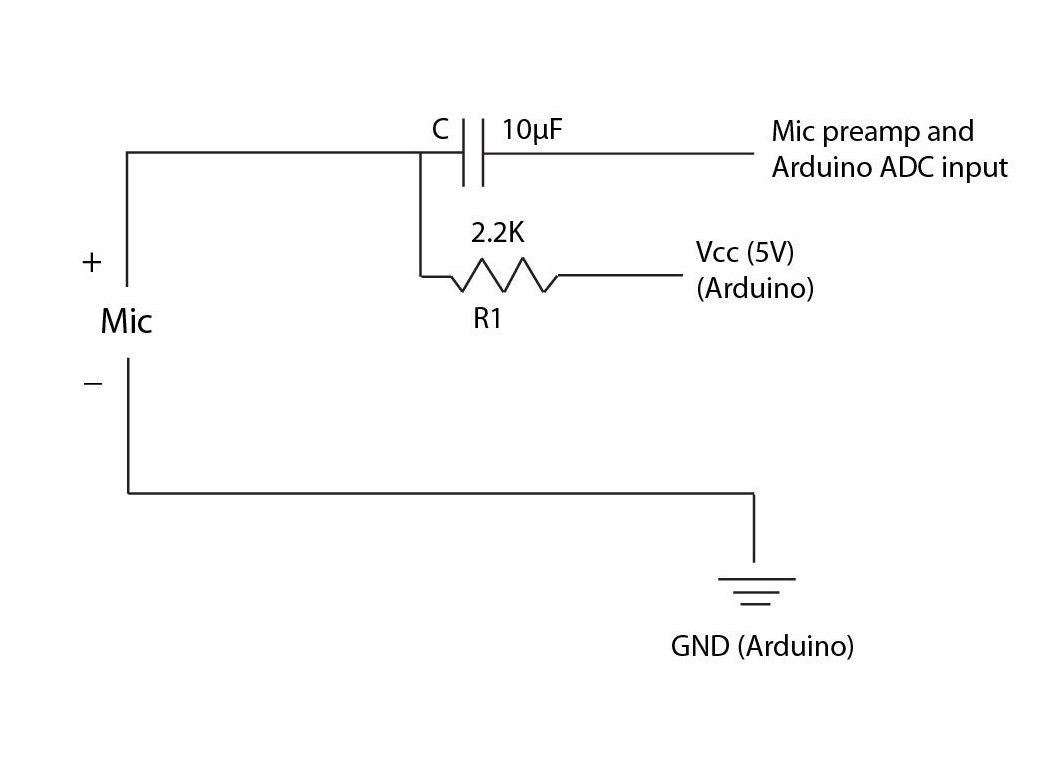
\includegraphics[width=1\textwidth]{micschem}
		     \caption{The schematic for each microphone wiring, from the MAKE article by Tristan Shone}
		\end{figure}
		
The device fulfills two roles: it can act as a controller through the use of the Arduino system and its MIDI generating code (Shone uses the HIDuino firmware to facilitate this), and also provide sound samples to 
	
We see a trend in the systems being presented here: simple electronics, serving a specific purpose between exploration of a physical process (touching in the case of Cihan's \emph{Porcupine}, voice in the case of Shone). Both represent instances of post-optimal approaches to interfaces through an exploration of the materials they use everyday. 
	
The Headgear is not the main element of Shone's live setup, nor is it necessarily its centerpiece. However, through its dual operating mode, the sharing of its design on public platform such as MAKE magazine, and the relative simplicity of its inner workings, it serves as a good example of the few things needed by an accomplished fabricator and artist to make a compelling device. 

As can be expected in parallel with the rise of microcontrollers as interfaces for turning our environment into a source of control data, recent years have seen a number of initiatives turning accessible, general purpose computing devices into code-based synthesis engines. All these projects are the embodiment of their designer's curiosity, adapted to various degrees of interactivity for performance, composition or commercialization. 

\section{Dan Snazelle: Snazzy FX}

Dan Snazelle is a recording engineer turned hardware designer. Although his relationship with musical electronics is mostly done through the design of analog electronics, he is one of the first to market an Arduino as the central piece of a synthesizer module. In doing so, Snazelle and his collaborator Darwin Grosse take advantage of the fast-paced communal activity of coding communities and the ability to sell a product even though there is enough information for people to build them from scratch. 

\subsection{The \textit{Ardcore} (2011)}

The Ardcore is in effect a reprogrammable lo-fidelity oscillator and control voltage generator packaged in a eurorack format and complemented by a set of freely available and editable programs. 

This project was developed by Darwin Grosse and Dan Snazelle. Darwin Grosse is a developer at Cycling `74, while Dan Snazelle is the owner and designer at Snazzy FX. Just like the Porcupine, the Ardcore documentation isn't all neatly packaged in a tutorial form, but a significant amount of  information is available for the curious. 

At the beginning of this project is Grosse's master's thesis at University of Colorado, Boulder. The document describes the first completed prototype and provides context, code examples, an overview of its possibilities, and detailed documentation of the collaboration process with Dan Snazelle. 

Of interest here is the information available to the tinkerer that might be interested in building their own homemade ardcore. Grosse's statement of purpose can be found in Appendix A of his thesis: 

\begin{quote}

	This specification provides the analog modular community with a standardized use of the Arduino microcontrollers system, and will include a large number of example sketches (programs) that accomplish tasks within the modular world. Any Arduino user can utilize these specifications to create modules, control systems or computer interfaces, and will be able to use any programs that others may come up with.
	
	\end{quote}
	
	\citep{grosse2011}
		
		\begin{figure}[H]
		  \caption{The Ardcore's first version circuit board, with an Arduino nano, by Darwin Grosse. Courtesy of Grosse}
		  \centering
		    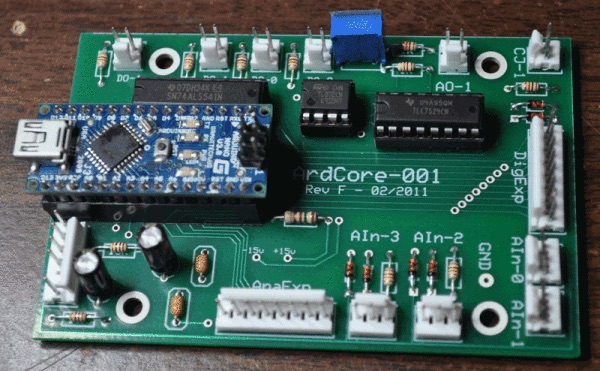
\includegraphics[width=1\textwidth]{ardcorev1}
		\end{figure}
		
		\begin{figure}[H]
		  \caption{The Ardcore's first version synthesizer module, by Darwin Grosse, courtesy of Grosse}
		  \centering
		    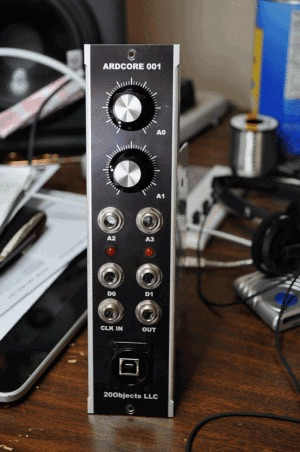
\includegraphics[width=1\textwidth]{ardcoremodule}
		\end{figure}
		
		\begin{figure}[H]
		  \caption{The Ardcore's current commercial package, by Snazzy FX, courtesy of Dan Snazelle}
		  \centering
		    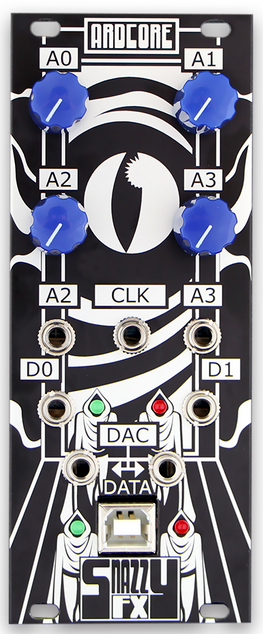
\includegraphics[width=.2\textwidth]{ardcoresnazzy}
		\end{figure}

Undertaking this project from scratch is somewhat more ambitious than any of the previous case studies. Because the Arduino code is all shared on Github, the software is not an issue, which is in line with the practices of the Arduino community. However, there doesn't seem to be any explicit tutorial or consolidated documentation for copying the hardware. Grosse's thesis details the development and manufacture in much detail, but never explicitly permits copies or provides a full schematic \citep[pp.21-31]{grosse2011}. 

		\begin{figure}[H]
		  \caption{The schematic for the DAC section of the Ardcore, based around a TLC7524, courtesy of Grosse}
		  \centering
		    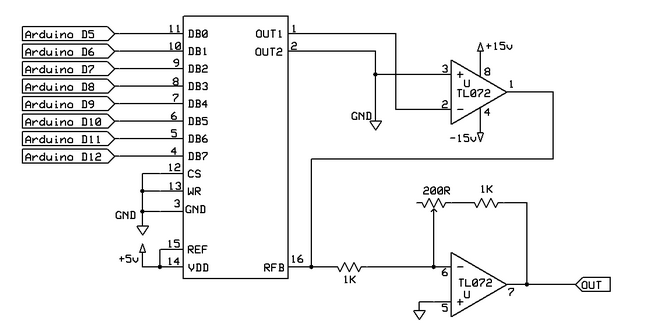
\includegraphics[width=1\textwidth]{ardcoredac}
		\end{figure}
		
		\begin{figure}[H]
		  \caption{The circuit board layout for the first version Ardcore, by Darwin Grosse}
		  \centering
		    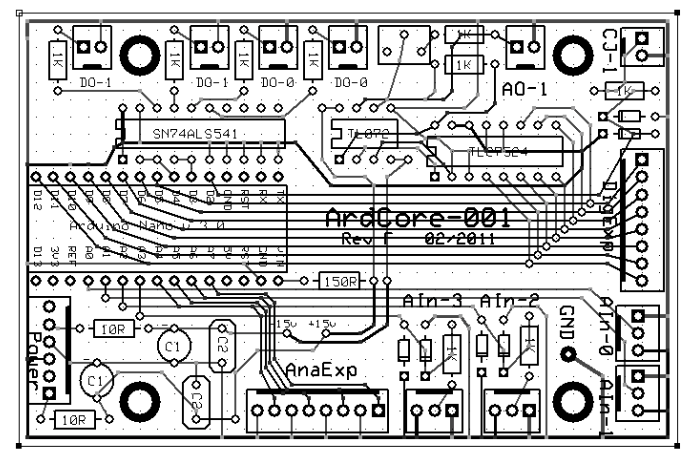
\includegraphics[width=1\textwidth]{ardcorepcb}
		\end{figure}

These documents do go a long way illustrating Grosse's preliminary design. Put briefly, the clocking input is implemented on a digital pin, while the analog out is done through eight other digital pins being connected to a TLC7524 digital to analog converter (DAC). All the voltage scaling necessary for the circuit to be functional with other devices in the modular environment (Grosse chose the one volt per octave standard) was done through the use of a TL072 op amp circuit with an internal trimpot calibration. The Arduino processor (the Atmel chip documented previously) can now serve as an in/out device for audio signal (albeit sampled at a low resolution of 8 bits) and produce voltages conforming to other manufactured modules. 

As Grosse and Snazelle finalized the eurorack version of the module, it becomes clear that the focus is this device's ``lo-fi swiss army knife of modular'' versatility. The ATmega chip at the center of this design not being meant for audio synthesis or real-time audio signal processing, this system offers plenty of limitations, gentle provocations and user-unfriendliness that qualify it as having post-optimal aspects. Unique to the ardcore, however, is that the two developers contribute actively to various repositories for newt module codes and application, with over sixty options easily available and a theoretically infinite variety of possibilities \citep{ardcode, ardcodeb}. 

The Arduino can be viewed as one of the driving force in making and artistic tinkering today \citep{gibb2010}. Integrating in a nostalgia medium such as the modular synthesizer system is both beneficial for the life-span of both items and for maintaining the relevancy of a founding technology in electronic music. By placing both their future in the hands of an open enthusiastic community, Grosse and Snazelle arguably guarantee both of their survivals.  

\section{Martin Howse}

Martin Howse is a British artist residing in Berlin and teaching workshops all over the world. Please refer to appendix A for additional information concerning his background and inspirations. 

Although not limited to this framework, Howse's technological experiments often fall within what he calls \emph{psychogeophysics}, which were defined in the anonymous \emph{Psychogeophysics Handbook \& Reader}: 

\begin{quote}
	
	Where does execution (of software) as an act take place and what are the effects of such sitings on the individual? Is there a stark division between the physical and the protocol (between the material and the symbolic), or can these terms be considered as points on a continuum of abstraction? Psychogeophysics attempts to answer these questions using a core methodology based around the pairing of paranoiac detection (parody of scientific practice) and excitation as intervention.
	
	\end{quote}
	
	\citep{anonymous2011}
	
This poetic exploration of technology as a parody of scientific practice appears about as nonsensical as \emph{experimental engineering}, and yet, Howse's work is not without recognition. Discussing Howse's performance work, Douglas Kahn writes: 
	
\begin{quote}

When he raised his hand and dug it into the soil, into the earth, a whole new battery of sounds were heard. It was phenomenal. Electricity always seeks a ground; he had grounded electronic music. It was more than a gesture; it was an epiphany.
\end{quote}

\citep{kahn2014}

This is another incarnation of what Dunne envisioned as effective post-optimality in design. Howse doesn't appear more as an engineer than musician, teacher, artist or theorist, rather, the easiest way to talk about him is on his own terms: as a psychogeophysicist.  

\subsection{The \textit{Dark Interpreters} (2013-ongoing)}

The dark interpreters is a series of ARM processor-based synthesizers. They come in three versions, the \emph{Mater Lachrymarum}, the \emph{Mater Suspiriorum}, and the \emph{Mater Tenebraum}. Each correspond to more complex versions of the same basic resampling / granulation synthesis processes, and all are available for purchase from Howse's website (http://www.1010.co.uk/org/darkint.html). 

All the files used by Howse to manufacture these circuit boards (schematics, layout, code) are available from his Github repository \citep{howse}. The hardware documentation is provided in the form of KiCad files, while a collection of C-based ARM code with comments details the functioning of the software. Howse's documentation requires a close look at best. Intentionally making a full understanding of the devices a bit more difficult suggests that post-optimal objects can be achieved through documentation as well. 

	\begin{figure}[H]
	  \centering
	    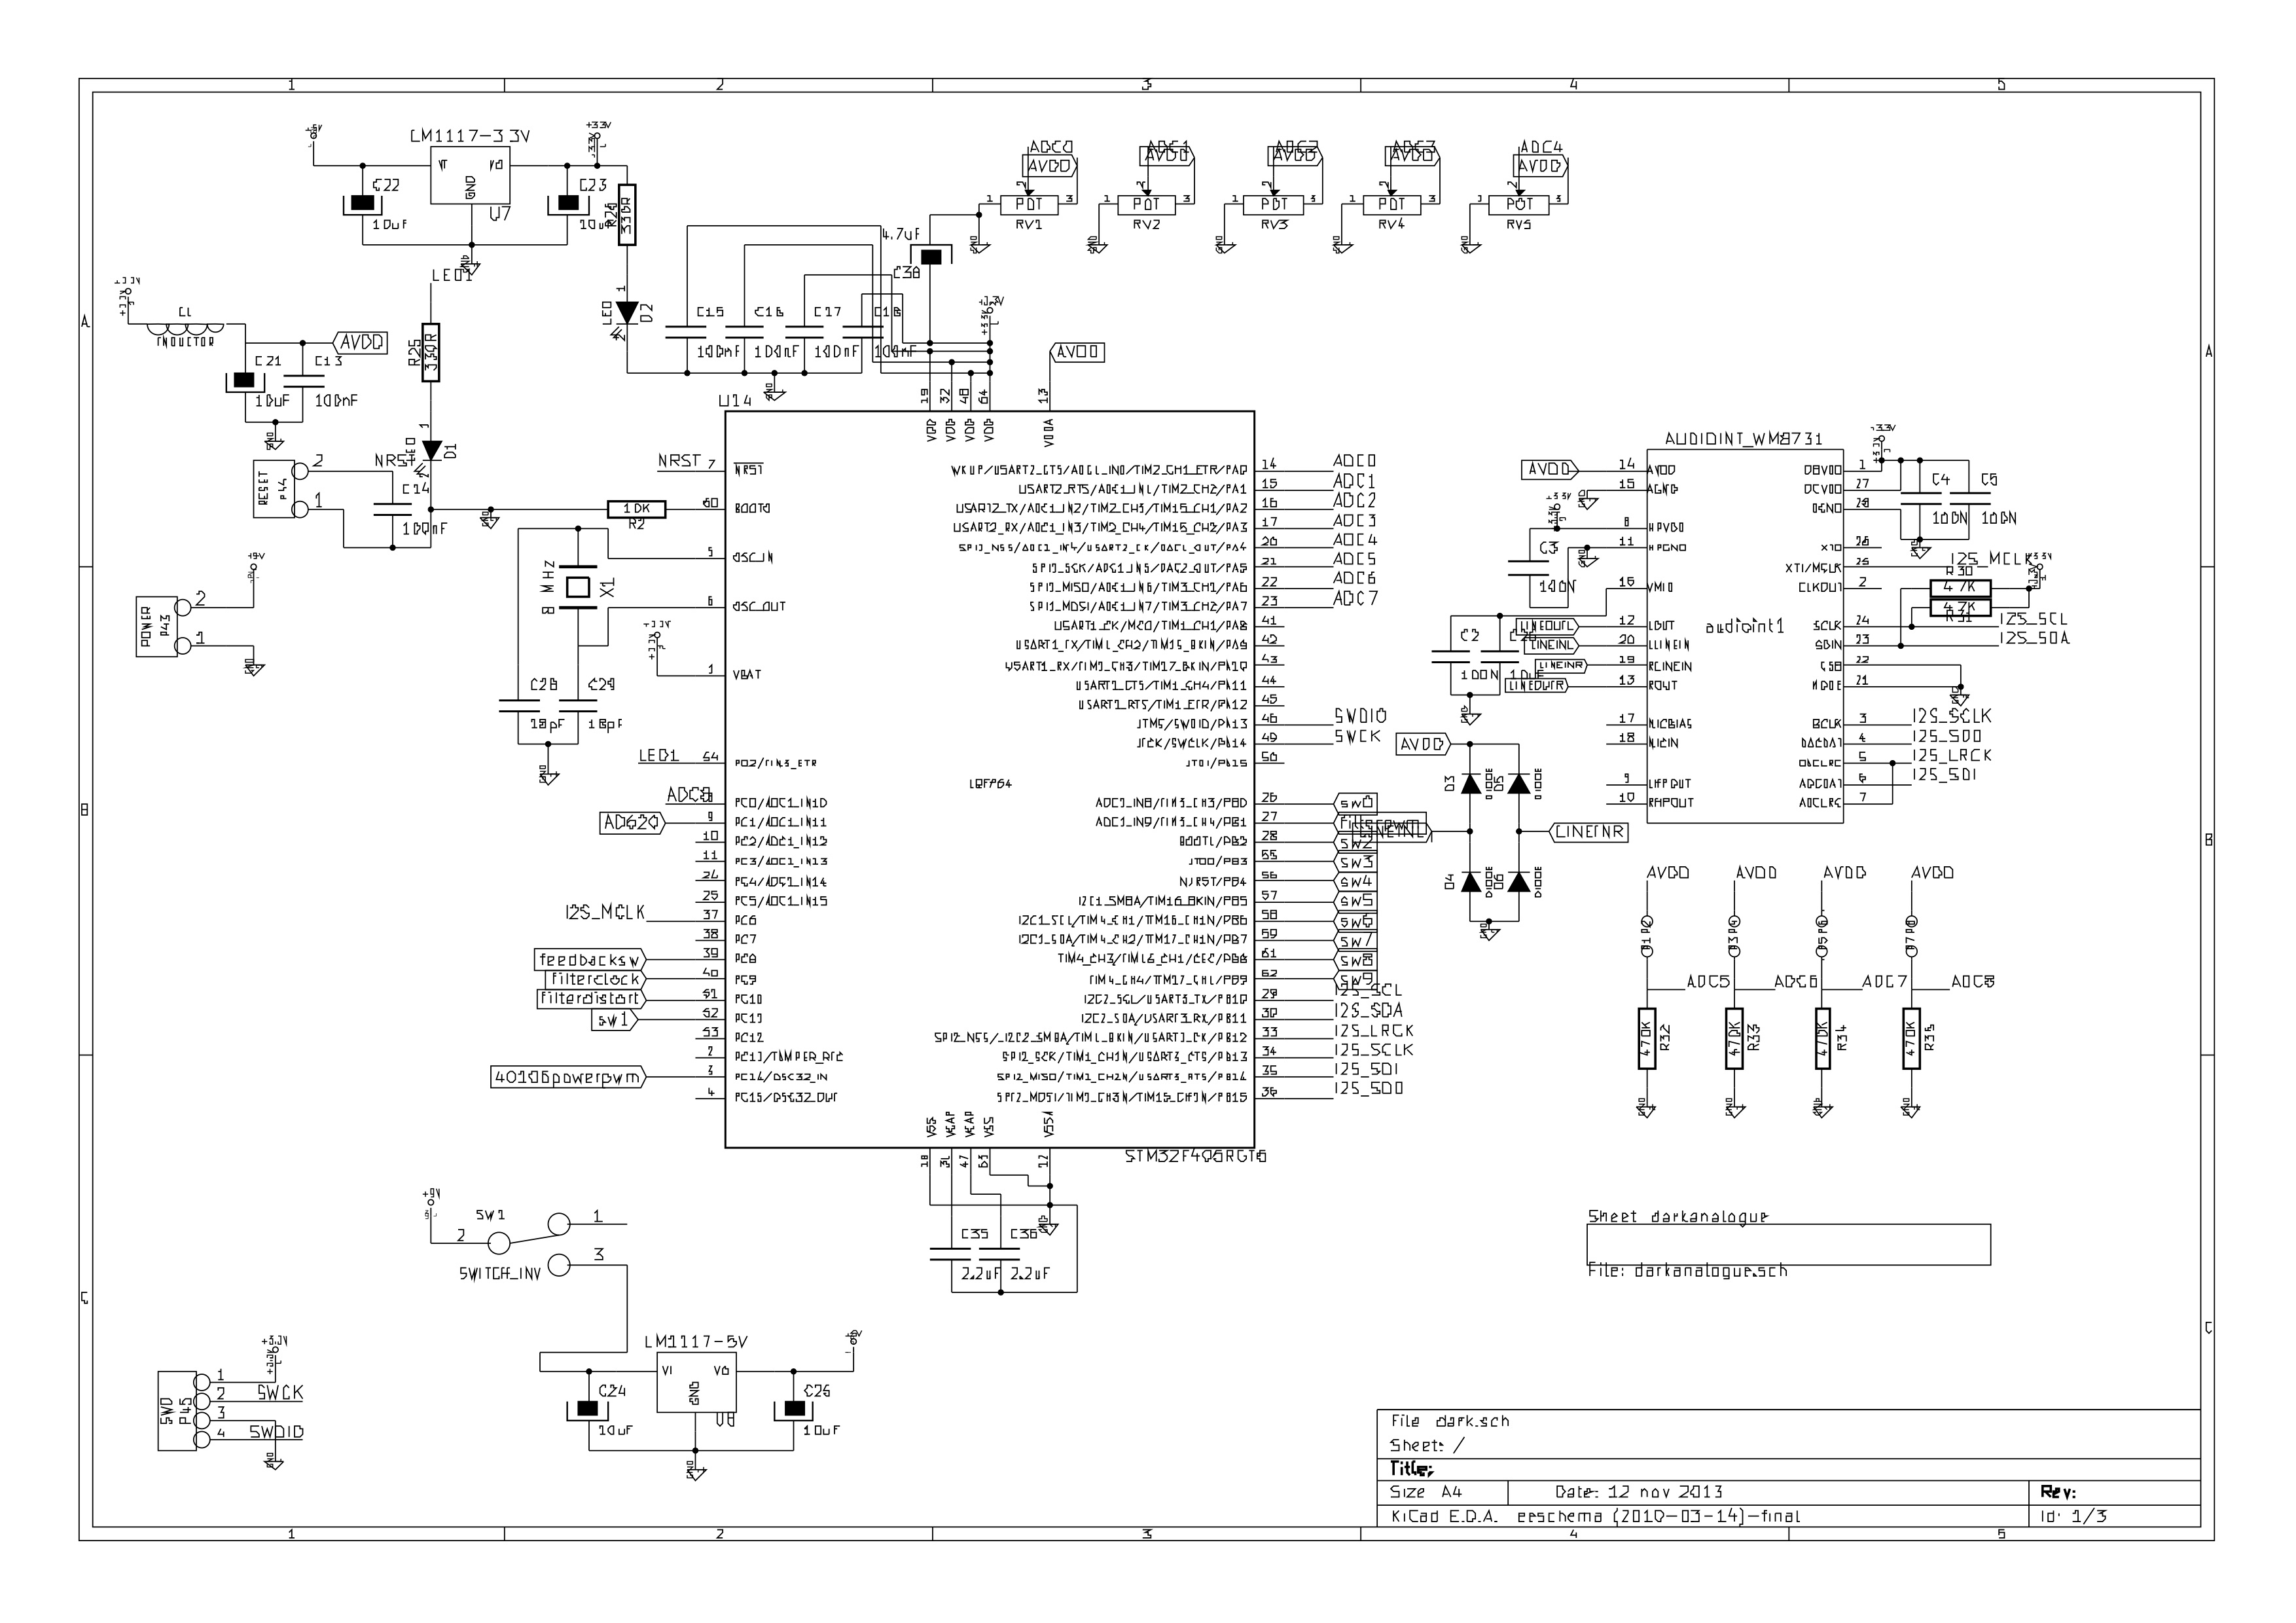
\includegraphics[width=1\textwidth]{mater1}
	    \caption{The schematic for the \textit{Mater Tenebraum}'s analog circuitry, courtesy of Martin Howse}
	\end{figure}
	
	\begin{figure}[H]
	  \centering
	    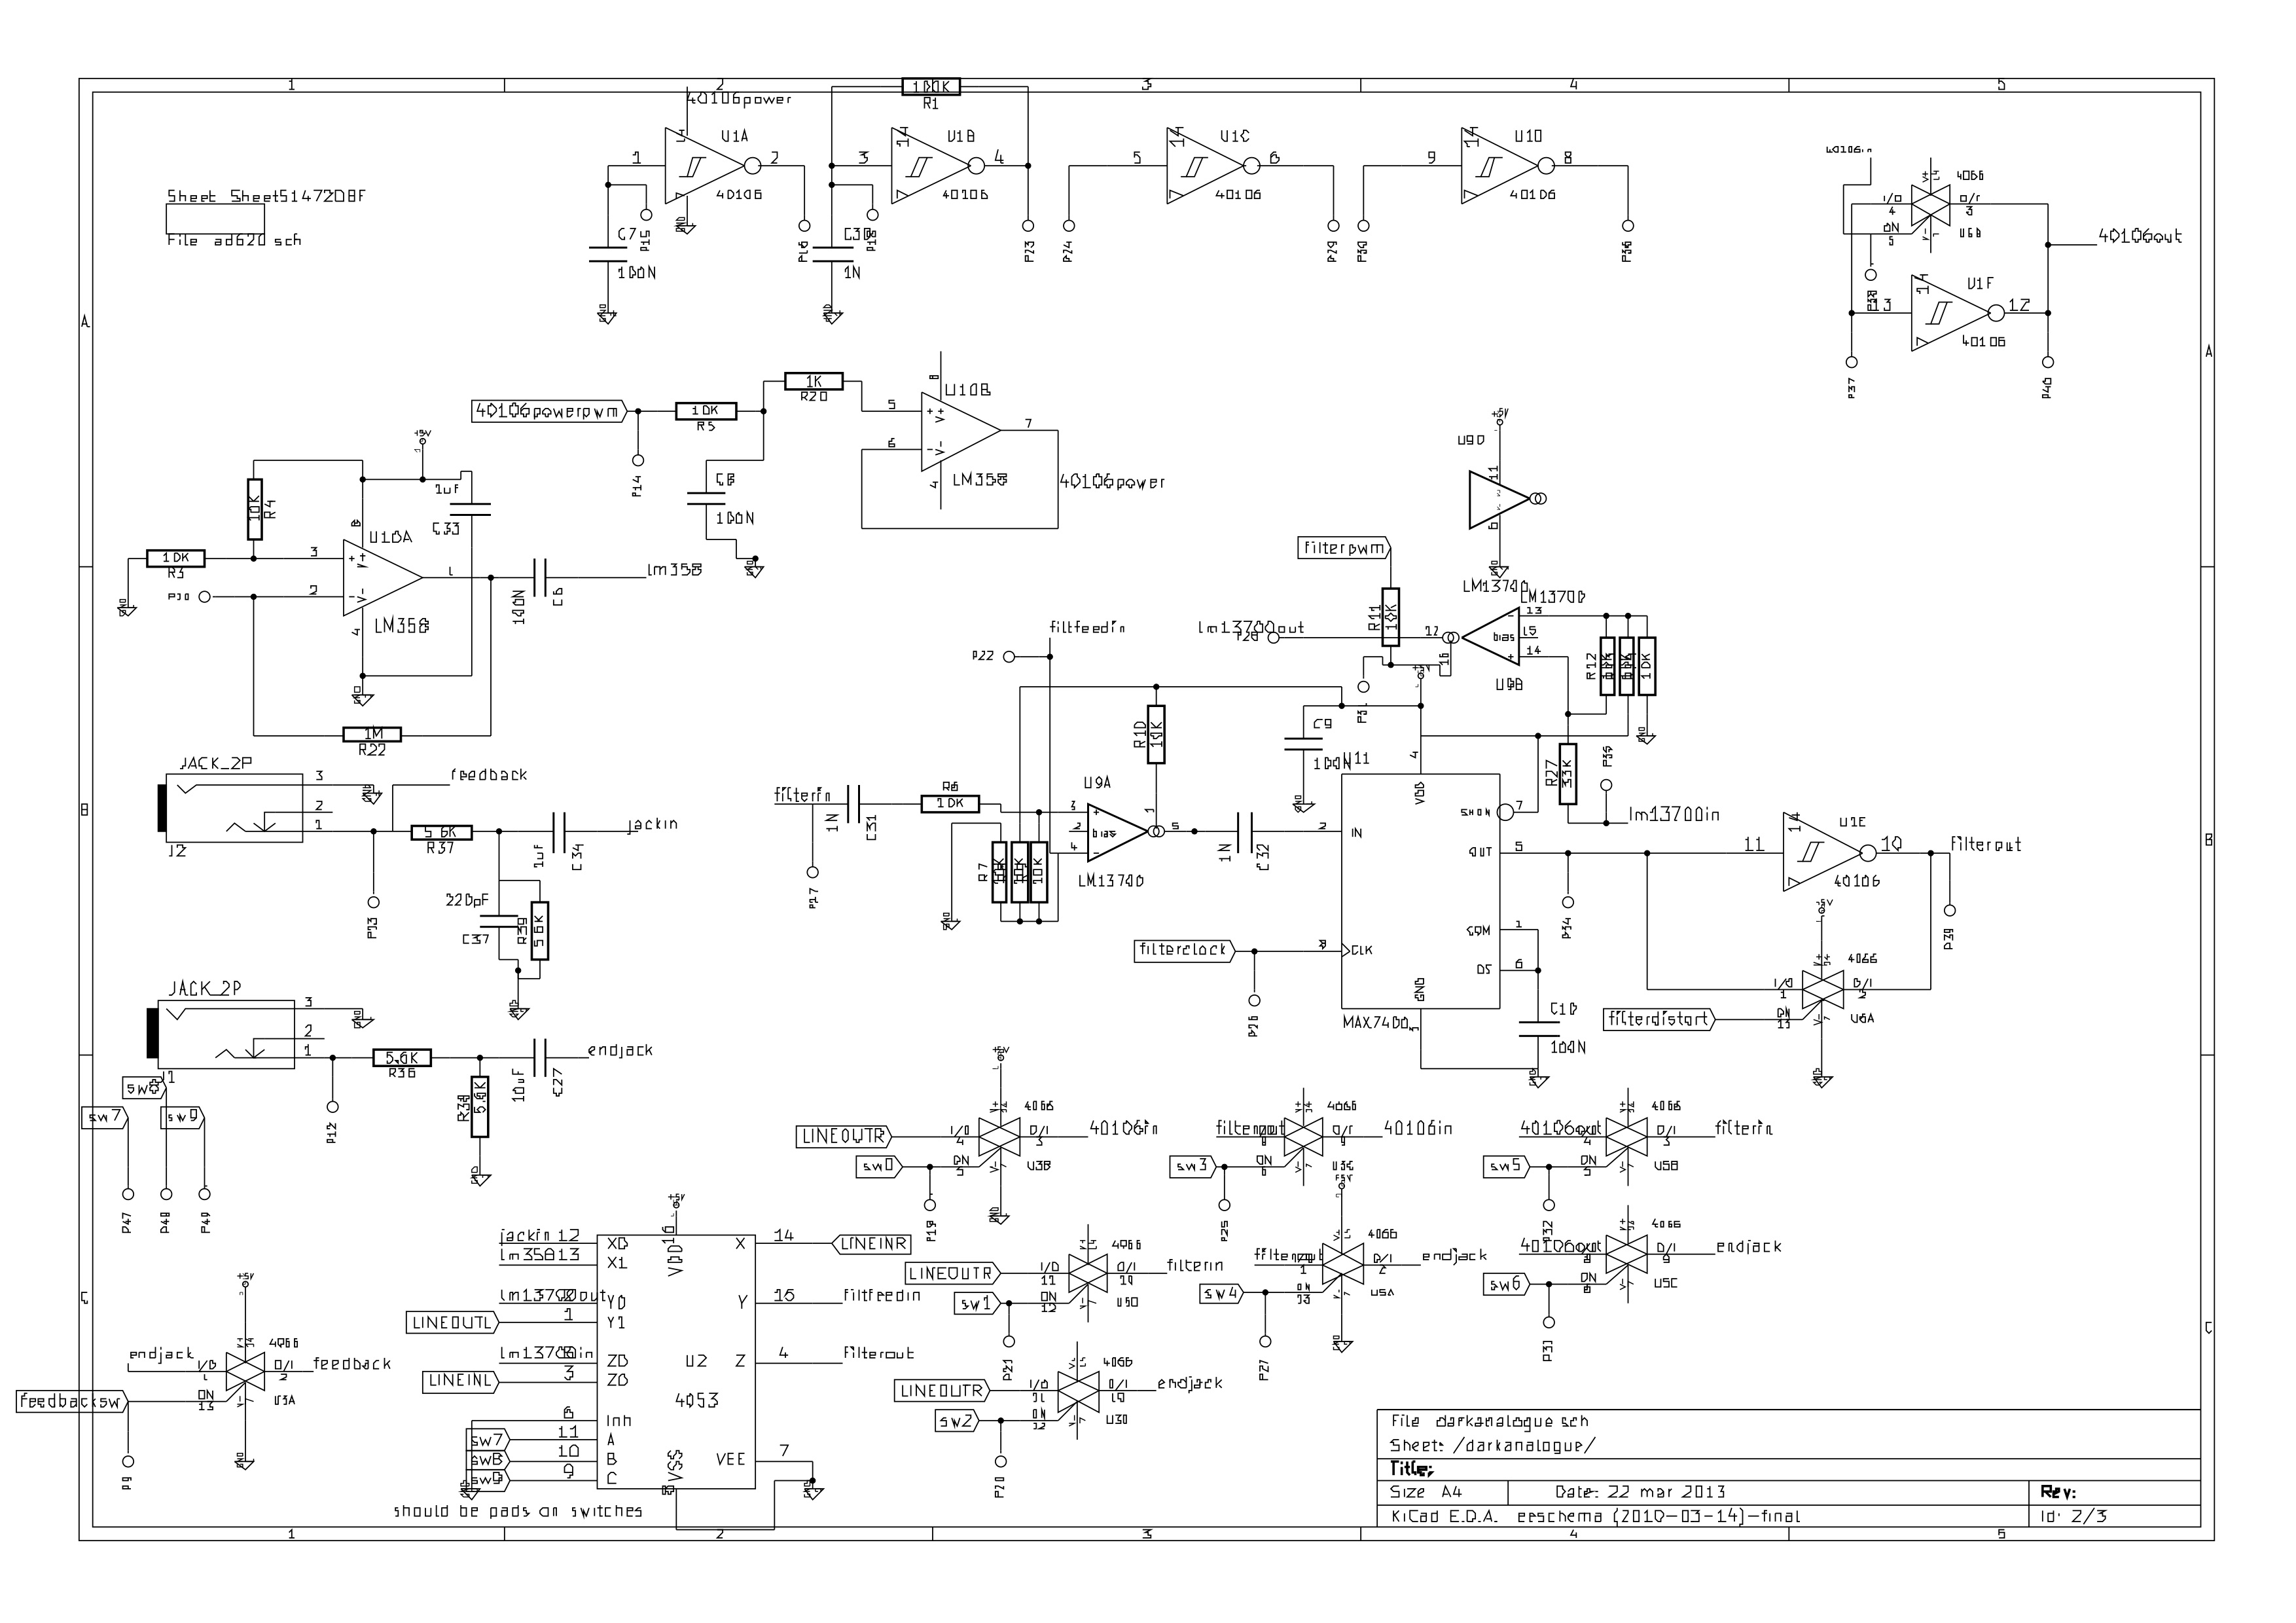
\includegraphics[width=1\textwidth]{mater2}
	    \caption{The schematic for the \textit{Mater Tenebraum}'s digital circuitry cou}
	\end{figure}
	
The manual provided by Howse details basic operation: 

\begin{quote}

The Dark Interpreter is modeled as a leaky, overlapping medieval village space within which various plague simulations run, and through which an array of villagers wanders. Audio is processed and/or generated according to the state of the village and the movements of inhabitants. Villagers (grains?) generate changes and are classified according to incoming or outgoing audio (read/write), filter, effects and hardware.

The Dark Interpreter is essentially mode driven, with modes also changing the complexity of operation. Modes are selected by turning knob 5. To set parameters in each mode a finger must be placed on the directions and then settings can be changed with knobs 1,2,3 and 4. Finger pressure/electricity determines speed of the villager’s movements or general mode speeds and the selected/fingered direction sets direction.

More advanced modes swap parameters between sets of villagers, allow for fingers to be placed right into code and parameters and finally allow for mirroring which sets selected parameters under the control of a selected mirror (the head/EEG board, the knobs, the fingers or the village itself).

\end{quote}

\citep{howse2015}
	
	\begin{figure}[H]
	  \centering
	    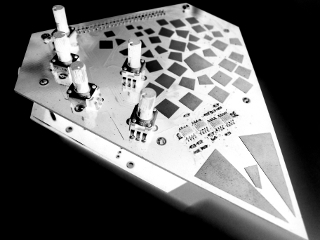
\includegraphics[width=.5\textwidth]{tenebraum}
	     \caption{The \textit{Mater Tenebraum}, with its copper pad interface and irregular shape. courtesy of Martin Howse}
	\end{figure}
	
Howse's constant contextualization of technical processes within a narrative framework (here, a plague influencing the interaction of villagers as a model for granular synthesis) is a fairly clear example of what Dunne could have meant by post-optimal devices as catalysts for poetic experiences of technology. Howse's backing in literature and conceptual art seems to guarantee that his technical work is grounded in those very poetic processes. 

This vision is however not contradictory with technological acuity. Looking at the source code and schematics shows a thorough understanding from the author of the goal and methods: 

\begin{figure}[H]
	  \centering
	    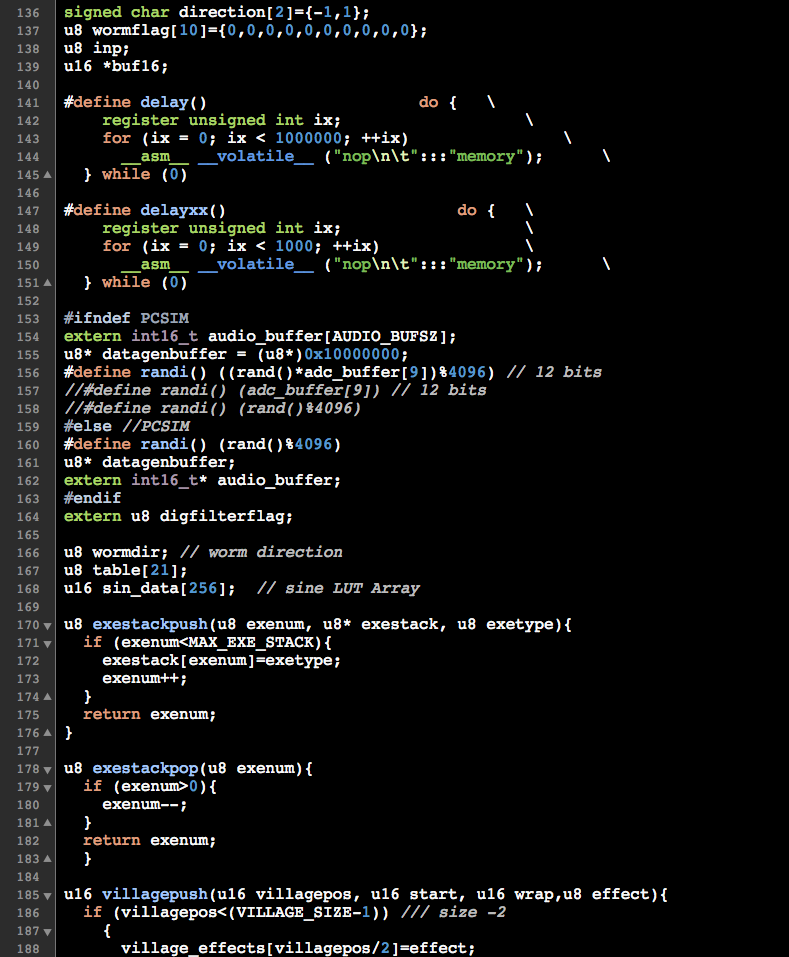
\includegraphics[width=1\textwidth]{codemater1}
	    \caption{A screenshot of the main.c file embedded in the \textit{Mater Tenebraum} courtesy of Martin Howse.}
	\end{figure}

The main code defines the granular synthesis engine, where each granule is presented as a villager living in a plague-ridden environment. 

\begin{figure}[H]
	  \centering
	    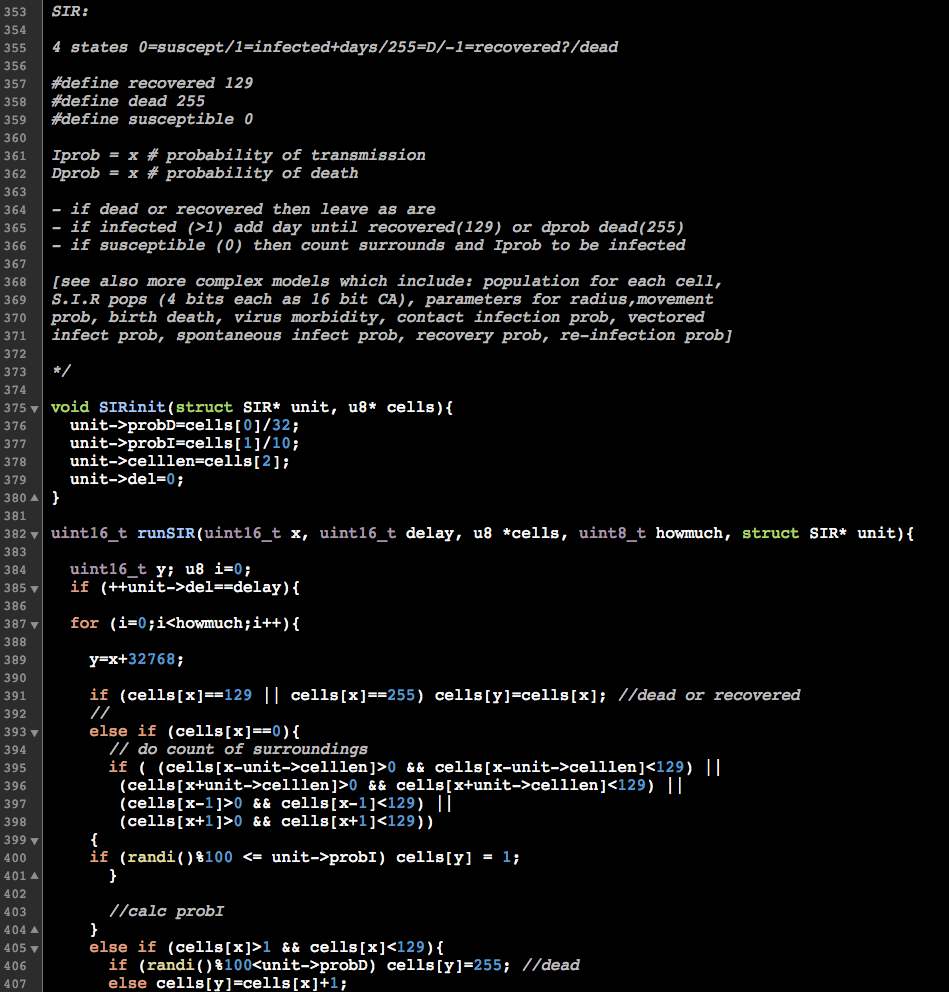
\includegraphics[width=1\textwidth]{codemater}
	    \caption{A screenshot of the CA.C embedded in the \textit{Mater Tenebraum} courtesy of Martin Howse.}
	\end{figure}
	
A cellular automata algorithm then describes the rules with which these granules interact, multiply and die. The plague is modeled using a classic suspected, infected, recovered (SIR) model. 

On the hardware side, one might notice that the 4000 series of CMOS chips is once again present (the 4053 triple multiplexer/demultiplexer, the 4066 quad analog switch, and the ever-ubiquitous 40106 hex Schmitt trigger). The embedded digital system is based around an ARM Cortex M4 chip that implements 16 bit, 48 kHz digital sampling as a basis for grain generation that can be heavily effected through under-sampling. 

\begin{figure}[H]
	  \centering
	    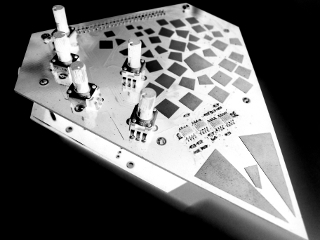
\includegraphics[width=1\textwidth]{tenebraum}
	     \caption{The \textit{Mater Tenebraum}, with its copper pad interface and irregular shape. courtesy of Martin Howse}
	\end{figure}

To recapitulate, the \emph{Dark Interpreters} are important in the context of a homemade electronic music because they: 

- serve as proof that a designer can effectively blend code and poetics in hardware 
- illustrate an interpretation of Dunne's \emph{post-optimal} objects through a unique interface and unpredictable use of the body or soil as circuit components
- demonstrate that publicly sharing source code and schematics does not necessarily take the mystery and interest away from the original designer's product
- offer another direct link between micro-computing systems and their logical ancestors, the CMOS 4000 series

\section{Sang Wook ``Sunny'' Nam \& Joshua Florian: mastering studio}

Sang Wook Nam is a mastering engineer teaching at Dartmouth College and running a mastering studio at the time of this writing \citep{nam2015}. As a mastering engineer, Nam does not manufacture synthesis or signal processing hardware. His connection to music technology is presented here because it serves as a fitting conclusion to our lineup of hardware examples: even in professional, closed source environments, open design methods and its products are important. 

In visiting his studio, it appears that most items in his setup fall within standard categories of equipment: channel selectors, equalizers, amplifiers, high quality analog to digital / digital to analog converters, etc. However, it also becomes clear that all of this equipment is custom made to satisfy Nam's trained and precise ear. 

	\begin{figure}[H]
	  \centering
	    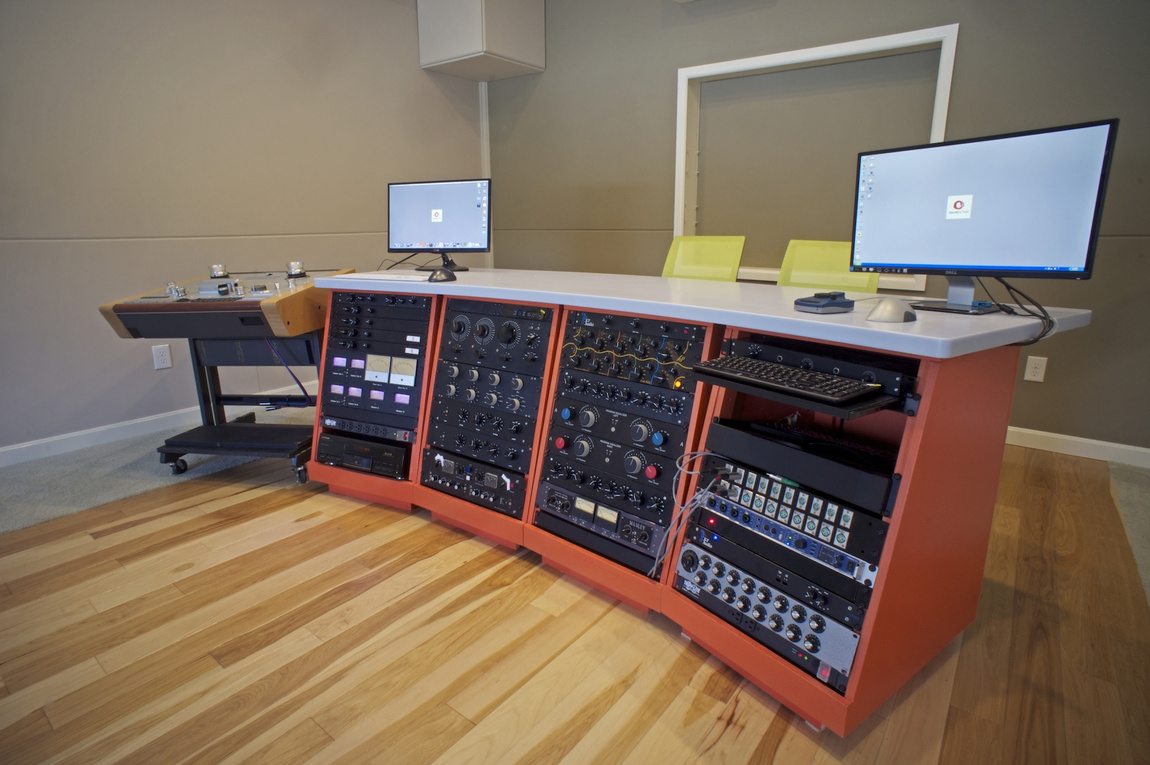
\includegraphics[width=1\textwidth]{sunnystudio}
	    \caption{The Jacob's Well mastering desk, courtesy of Sang Wook Nam}
	\end{figure}
	
Most of this equipment is designed, assembled and tested in collaboration with JCF audio's founder and owner, Joshua Florian \citep{florian2015}. After Nam and Florian worked together at LA's Mastering Lab, Nam came to value Florian's understanding of what they describe as ``yestertech'' \citep{florian2015b}: older audio hardware circuit designs, usually discrete semiconductor or tube, that were used in high end recording and mastering studios along with the rise and heyday of major labels. A number of parts in Nam's current setup come from A\&R mastering studio, which he purchased when they closed down. 

This section does not contain a particular product description. However, the concept of ``yestertech'' is deeply related to that of post-optimal objects and design methodology in electronic music hardware. As Nam's collaborator Joshua Florian mentions, designs respectful of yestertech use a personal and variable tool to measure success: human hearing. A significant portion of his work is to refine previously successful audio circuits, occasionally updating them to use new parts or to accommodate for the disappearance of an obsolete component. Engineering methodology is still an important part of the process, considering that many of the highly-respected audio amplifier and filtering designs are from professional or retired aerospace and defense contractors, but  this appreciation of older topologies and skepticism towards the latest products, yestertech in effect is an approach to post-optimal audio electronics. 

\section{Comments}

\begin{quote}
	
	My favorite programming language is... solder. 
	
	\end{quote}
	
	Robert Pease (1940-2011)

One case-study that was considered for this section concerned the performance practice of a small group, Live Objects. They were not included because their point, although crucial, was short: connecting engineering to performance art is more than possible, it can be desirable. 

In some of the case-study this chapter does include, the performative aspects of each practitioner's process or use of the devices was clear, but none merge design and musical performance as closely as Live Objects. 

The technology they use is largely similar to the above case-studies, using preprogrammed microcontrollers and slowly connecting them to additional parts to derive complex musical structure from circuits small and versatile enough to be assembled as part of a standard-length performance. One of their members is Tristan Perich, who has been garnering recognition for his highly deterministic preprogrammed code-based scores, which specify a performance in ways directly indebted to western musical thinking and notation. 

However, in the context of Live Objects, the group members take on a radically different approach, submitting the mechanic precision of digital electronics to the whims and inconsistencies of not just humans, but also of solder, wire, batteries, etc. Acknowledging the very material reality of computing devices \emph{in real time} is still somewhat original: post-optimality shows artistic promise in music beyond simple devices. 

To conclude, this section formally analyzed the information openly available to describe a set of devices that shared post-optimal aspects. To better understand the motivations behind these alternative approaches, the upcoming chapter presents discussions with some of the authors of these devices and associated practitioners. 

